\documentclass[10pt]{scrreprt}

% quick TOC setup
\KOMAoption{toc}{chapterentrydotfill}
% don't use parskip package, set parskip=full instead
\KOMAoption{parskip}{half}

\usepackage[twoside
            ,papersize={148mm, 210mm}
            ,layoutsize={148mm, 210mm}
            ,top=1.5cm
            ,bottom=2cm
            ,footskip=1cm
            ,textwidth=12cm
            ,verbose
            ]{geometry}

% \renewcommand*{\chapterheadstartvskip}{}

\usepackage[english, ngerman]{babel}

\usepackage{graphicx}
\usepackage{fancyhdr}
\usepackage{eso-pic}
\usepackage{caption}
\usepackage{wrapfig}
\usepackage{menukeys}
\usepackage{amssymb}
\usepackage{eurosym}
\usepackage{multicol}
\usepackage{lscape}
\setlength{\multicolsep}{0.5em}
\usepackage{adjustbox}
% fancy fone awesome boxes
\usepackage{awesomebox}

% mainly for linklist
\usepackage{longtable}
\usepackage{enumitem} % to easily remove itemize indent for the checklist

\usepackage{pdfpages}
\usepackage{fontspec}
\usepackage{microtype}
\usepackage[autostyle=true]{csquotes}
\MakeOuterQuote{"}

\PassOptionsToPackage{hyphens}{url}
\usepackage[colorlinks=false, pdfborder={0 0 0}]{hyperref}


% \definecolor{ese_bg_color}{rgb}{0.0, 0.20, 0.376} % the definitive color -- #003360 (2015?)
% \definecolor{ese_bg_color}{rgb}{0.0, 0.263, 0.486} % the definitive color -- #00437C (2016?)
% \definecolor{ese_bg_color}{rgb}{0.051, 0.373, 0.596} % the definitive color -- #0D5F98 (2017)
% \definecolor{ese_bg_color}{rgb}{0.796, 0.376, 0.251} % the definitive color -- #CB6040 (2018)
% \definecolor{ese_bg_color}{rgb}{0.0, 0.47, 0.3} % wip-ish color -- #01794C (2019)
% \definecolor{ese_bg_color}{RGB}{5,109,133} % final_really_final -- #056d85 (2020)
\definecolor{ese_bg_color}{RGB}{155,30,70} % complement -- #9B1E46 (2021)
\definecolor{ese_fg_color}{rgb}{1, 1, 1}

\definecolor{fancypageref_color}{RGB}{155,30,70} % 

\definecolor{ifsrgray}{rgb}{0.6, 0.6, 0.6} % 153, 153, 153

% is toggled twice for moduluebersicht.tex
\changemenucolor{gray}{bg}{named}{ese_fg_color} %background of the menukeys
\changemenucolor{gray}{br}{named}{ese_bg_color} %border of the menukeys
\changemenucolor{gray}{txt}{named}{ese_bg_color} %text of the menukeys

\setmainfont[
  Scale=0.90,
  BoldFeatures={Scale=1.0}
]{Open Sans}

\setmonofont[
	Scale = 1.09
]{Latin Modern Mono}

\setkomafont{chapter}{\color{ese_bg_color}\fontspec[BoldFont={* Bold}]{Open Sans}\huge\bfseries}
\setkomafont{minisec}{\color{ifsrgray}\fontspec[BoldFont={* Bold}]{Open Sans}\large\bfseries}
\setkomafont{paragraph}{\color{ifsrgray}\fontspec[BoldFont={* Bold}]{Open Sans}}
\setkomafont{pagenumber}{\color{ifsrgray}\fontspec{Open Sans}}

\addtokomafont{disposition}{\normalfont\fontspec{Open Sans}}
\defaultfontfeatures{Ligatures=TeX}  % enable ligatures (e.g. --) for new fonts


\newcommand{\ascii}{{\texttt{ascii}}}
\newcommand{\bafog}{BAföG}

\newcounter{linkcounter}
\newcommand\linklist{}
\makeatletter
\def\@breaklinklistat{22}
\def\@breaklinklistandat{54}
\newcommand{\link}[1]{%
    \edef\tmptoken{\detokenize{#1}}%
    \@ifundefined{nopanic@link@\tmptoken}{%
        \edef\@linknumber{\arabic{linkcounter}}%
        \protected@edef\@tmpkey{{\fontsize{9pt}{0}\selectfont\keys{\@linknumber}}}%
        \expandafter\global\expandafter\edef\csname nopanic@link@\tmptoken\endcsname{\arabic{linkcounter}}%
        %
        % Standard print output:
        \expandafter\g@addto@macro\expandafter\linklist\expandafter{\@tmpkey & \url{#1}}%
        \ifx\@breaklinklistat\@linknumber
            \g@addto@macro\linklist{\\}%
        \else
            \ifx\@breaklinklistandat\@linknumber
                \g@addto@macro\linklist{\\}%
            \else
                \g@addto@macro\linklist{\\*}%
            \fi
        \fi
        %
        % Link system output:
        \immediate\write\linklistfile{RewriteRule "^\@linknumber$" "#1"}%
        %
        \stepcounter{linkcounter}%
    }{%
        \protected@edef\@tmpkey{{\fontsize{9pt}{0}\selectfont\keys{\csname nopanic@link@\tmptoken\endcsname}}}%
    }%
    \href{#1}{\@tmpkey}%
}
\makeatother


\hypersetup{
    pdfauthor={FSR Informatik der TU Dresden},
    pdftitle={The Manual - ESE \eseyear},
    breaklinks=true, colorlinks=false, pdfborder={0 0 0},
  pdfencoding=unicode
}

% we need this dummy counter to make a label at the spieleabendplakat
\newcounter{dummy}

\sloppy % forces "ugly" line breaks

\pagestyle{plain}

\begin{document}
%Das Coverbild, oh gott o.O Aber es funktioniert
\newcommand\CoverPic{%
\put(0,0){%
\parbox[b][\paperheight]{\paperwidth}{%
\vfill
\centering
\includegraphics[width = \paperwidth, height = \paperheight]{cover/Vorne}%
\vfill
}}}
\thispagestyle{empty} %keine Seitenzahl
\pagecolor{ese_bg_color}
\AddToShipoutPictureBG*{\CoverPic}
\mbox{} %brauche leeren Content für ne newpage
\newpage
\pagecolor{white}

% Linklist output
% All this stuff needs is immediate to avoid confusion between links on the same page
\immediate\newwrite\linklistfile
\immediate\openout\linklistfile=kopimi.htaccess\relax
\immediate\write\linklistfile{RewriteEngine On}
\immediate\write\linklistfile{RewriteBase /\eseyear}

\documentclass[a5paper,7pt]{scrreprt}
\usepackage[default]{opensans}
\usepackage[margin=0.55cm,landscape]{geometry}
% \usepackage[height=25cm]{geometry}
\usepackage{xcolor}
\usepackage{timetable}
\usepackage{transparent}
\usepackage{amssymb}
\usepackage{enumitem}
\usepackage{pifont}
\newcommand{\wontfix}{\rlap{$\square$}{\large\hspace{1pt}\xmark}}


\ifdefined\colormodel\relax\else%
    \def\colormodel{rgb}%
\fi
\selectcolormodel{\colormodel}

% \definecolor{ese_bg_color}{rgb}{0.0, 0.20, 0.376} % the definitive color -- #003360 (2015?)
% \definecolor{ese_bg_color}{rgb}{0.0, 0.263, 0.486} % the definitive color -- #00437C (2016?)
% \definecolor{ese_bg_color}{rgb}{0.051, 0.373, 0.596} % the definitive color -- #0D5F98 (2017)
% \definecolor{ese_bg_color}{rgb}{0.796, 0.376, 0.251} % the definitive color -- #CB6040 (2018)
% \definecolor{ese_bg_color}{rgb}{0.0, 0.47, 0.3} % wip-ish color -- #01794C (2019)
%\definecolor{ese_bg_color}{RGB}{5,109,133} % final_really_final -- #056d85 (2020)

\definecolor{ese_bg_color}{RGB/cmyk}{155,30,70/0,0.9,0.6,0.1} % complement -- #9B1E46 (2021)
\definecolor{ese_fg_color}{rgb/cmyk}{1,1,1/0,0,0,0}

\definecolor{fancypageref_color}{RGB/cmyk}{155,30,70/0,0.9,0.6,0.1} %

\definecolor{ifsrgray}{rgb/cmyk}{0.6,0.6,0.6/0,0,0,0.4} % 153, 153, 153


\begin{document}
\thispagestyle{empty}
% \begin{landscape}

% Define the layout of your time tables
\setslotsize{3.00cm}{0.25cm}
\setslotcount{6}{52}
\settopheight{2}
\settextframe{0.8mm}

% Retro
\setframetype[t]{1}
\seteventcornerradius{0pt}

% Print timestamps into event blocks
% \setprinttimestamps{2}

% Define event types
%background  foreground

\leteventcolors{ese}%
  {ese_bg_color}
  {ese_fg_color}
% Start the timetable
\begin{center}
\begin{timetable}
  \hours{8}{15}{0}
  \germandays{1}
  \event 1 {1000}{1630}{Wanderung}{}{HBF}{}{ese}{0}
  \event 1 {1800}{2100}{Spieleabend}{}{APB}{}{ese}{0}

  \event 2 {0920}{1100}{Begrüßung}{}{}{1}{ese}{0}
  \event 2 {1130}{1300}{Tutorien}{}{APB/WIL/SCH}{1}{ese}{2}
  \event 2 {1130}{1300}{Master\\How-to}{}{}{}{ese}{1}
  \event 2 {1300}{1400}{gemeinsames Mensen}{}{}{}{ese}{0}
  \event 2 {1400}{1600}{Bunter Nachmittag}{}{}{}{ese}{0}
  \event 2 {1800}{1900}{Grillen mit Dewpoint}{}{Countdown}{}{ese}{0}
  \event 2 {1900}{2100}{Clubwanderung}{}{}{}{ese}{0}

  \event 3 {0830}{0900}{Frühstück}{}{}{}{ese}{0}
  \event 3 {0900}{1030}{Vortrag zum Studium}{}{}{}{ese}{0}
  \event 3 {1030}{1300}{Einschreibung}{}{}{}{ese}{0}
  \event 3 {1300}{1400}{Mittagessen}{}{}{}{ese}{0}
  \event 3 {1400}{1700}{Gemüseauflauf (Schnitzeljagd über den Campus)}{}{}{}{ese}{0}
  \event 3 {1800}{2100}{Filmabend}{}{KIK}{}{ese}{0}


  \event 4 {0900}{1100}{online\\Welcome\\session\\CMS}{}{}{}{ese}{1}
  \event 4 {0900}{1100}{Profvrstllng}{}{}{}{ese}{2}
  \event 4 {1100}{1300}{Vortrag Sprachkurse \& Auslandsstudium}{}{}{}{ese}{0}
  \event 4 {1300}{1400}{Mittagessen}{}{}{}{ese}{0}
  \event 4 {1400}{1530}{Kaffetrinken mit Nerds}{}{}{0}{ese}{0}
  \event 4 {1600}{1730}{Feierliche Imma}{}{}{}{ese}{0}
  \event 4 {1730}{1900}{Party}{}{HSZ Wiese}{}{ese}{0}
  \event 4 {2000}{2100}{Bowling}{}{}{}{ese}{1}
  \event 4 {2000}{2100}{Spieleabend}{}{}{}{ese}{2}

  \event 5 {0900}{1300}{Seminargruppentreffen \& Vortrag studentisches Engagement}{}{}{}{ese}{0}
  \event 5 {1300}{1400}{Mittagessen}{}{}{}{ese}{0}
  \event 5 {1400}{1700}{ESE Spiel}{}{}{}{ese}{0}
  \event 5 {1800}{2100}{Neustadt\\ Clubtour}{}{Albertplatz}{}{ese}{1}
  \event 5 {1800}{2100}{PnP}{}{APB}{}{ese}{2}
  
  \event 6 {0900}{1000}{Stadtführung}{}{siehe Website}{}{ese}{0}
  \event 6 {1700}{2100}{LAN Party}{}{siehe Website}{}{ese}{0}
\end{timetable}
\end{center}
% \end{landscape}
\end{document}

\include{texte/inhaltsverzeichnis}
\addchap{Was ist das hier?}


Hallo! Bis hierher hast du es nun schon mal geschafft. Wahnsinn!

Wie du vielleicht im Verlauf deines jetzt beginnenden Studiums feststellen wirst, ist es eine der schwersten Aufgaben, einen Informatiker zum Lesen des Handbuchs oder der Dokumentation zu bewegen. Vielleicht ist das so ein Spleen, der uns anhängt, vielleicht basteln wir aber auch einfach lieber tagelang an einem Problem, als eine halbe Stunde zum Nachschlagen im Handbuch zu investieren.
Oft wird euch deshalb in Foren oder bei StackOverflow der Satz entgegenschlagen: \enquote{RTFM} -- Read the fucking manual.

Aber die gute Nachricht ist, wenn ihr das hier lest, tretet ihr diesem Vorurteil schon mal entgegen. Denn dieses Heft ist ein kleines Handbuch für euer Studium.
Es verrät euch, wie die Uni funktioniert, Lehrveranstaltungen aufgebaut sind, ihr euch in Prüfungen einschreibt, was der Campus alles zu bieten hat und noch vieles mehr.
Wie jedes gute Handbuch enthält es dabei viel zu viele Informationen, die man kaum auf einmal brauchen oder verarbeiten kann.

Deswegen reicht es auch, wenn ihr euch jetzt beim Lesen auf alle mit \keys{must read} gekennzeichneten Kapitel beschränkt und den Rest später mal nachschlagt oder euch über die FAQ-Sektion auf Seite~\pageref{sec:faq} zu den passenden Antworten durchhangelt.
Dieses Buch ist so angelegt, dass es euch über den Großteil eures Studiums mit Informationen und Antworten weiterhelfen kann. Hebt es euch also auf und kramt es immer mal wieder raus. Wie jedes gute Handbuch :)

Und jetzt erstmal weg mit dem Schmöker! Dich erwartet die Erstsemestereinführung (ESE), die dir in der kommenden Woche erstmal das Wichtigste erklärt.
Genieß diese Zeit und mach dich bereit für die noch spannendere, die dich jetzt erwartet!

\textbf{Bleibt nur noch zu sagen: Viel Spaß in der ESE und im Studium!}

% \begin{figure}[b!]
% 	\centering
% 	\includegraphics[trim={0 5.5cm 0 0}, clip, width=\linewidth]{img/ese2015/bueroansturm.jpg}
% \end{figure}%

\begin{awesomeblock}[ese_bg_color]{2pt}{\faLightbulb[regular]}{ese_bg_color}
    \begin{minipage}[t]{.82\textwidth}
\small PS\@: Links schauen in diesem Heft so aus: \link{https://html5zombo.com}. Ganz hinten auf einer der letzten Seiten kannst du dann die Adresse nachsehen. Ebenfalls kannst du auch direkt unter \url{ese.ifsr.de/2022/<Zahl>} auf die verlinkte Seite weitergeleitet werden.
    \end{minipage}
\end{awesomeblock}

\addchap{Greetings}

\begin{wrapfigure}{l}{0.31\textwidth}
  \vspace{-12pt}
  \begin{centering}
    
\includegraphics[width=0.3\textwidth]{img/sbalzarini.jpg}
  \end{centering}
  \caption*{\copyright MPI CPG}
  \vspace{-15pt}
\end{wrapfigure}

{\fontsize{10pt}{11}\selectfont
\selectlanguage{english}
Dear Students,

a wholehearted \enquote{Welcome} to the Faculty of Computer Science at TU Dresden! Congratulations for having decided to study computer science our university, as no other course of studies would nowadays open so many doors and provide you with so many opportunities like ours, and TU Dresden provides you with an excellent environment to pursue your goals in one of Germany’s most livable and affordable student cities.

We are a diverse, international, and interdisciplinary community of about 2400 students (every third from abroad), 220 scientists, 222 registered PhD students, 28 professors, 4 Honorary Professors, and two independent Group Leaders with the status of \enquote{TUD Young Investigator}. Together, we are one of the top computer science departments in Germany. We offer a selection of nine degree programs, including two international Master’s programs entirely taught in English. These curricula cover the entire breadth of our exciting discipline. And we are fortunate to do so under excellent conditions with state-of-the-art infrastructure. Our department is housed in a modern building offering generous teaching rooms and well-equipped labs. We have access to some of the best high-performance computing resources of Germany with machines hosted in a dedicated building just next door. Finally, our university's sports facilities are located just behind our building, and the student-run café \ascii{} in the Lobby of our building is a focal point of our social life.

Our building is proudly named after Prof. Andreas Pfitzmann, who was our chair of privacy and security until 2010. Andreas Pfitzmann's work was not only scientifically noted, but his social engagement had far-reaching consequences for the public opinion and the lawmaking in Germany. Andreas Pfitzmann is partly responsible for the fact that the German public has an internationally unparalleled level of awareness when it comes to topics of data protection, security, and privacy.  This is just one example of how computer science directly impacts and shapes many areas of our everyday lives. A young discipline, computer science is unique in its blend of being both a structural science, like mathematics and philosophy, and an engineering discipline. It has revolutionized the way we communicate with each other, the way we run organizations, manage industrial production, and do science in almost all disciplines. There is almost no area of science, technology, or society that would not be shaped by and depend on advancements in computer science. Computing is a universal language that reaches far beyond tech geekery and hobbyist programming. It is theory and algorithms that provide a rigorous mathematical understanding of "information processing". It is human-machine interaction and the human in the loop, linking our discipline to psychology and the arts. It is the information processing that happens in living cells and organisms by chemical signaling pathways and the neurons in our brains, linking to systems biology and medicine. It is machine learning and artificial intelligence that aim to produce \enquote{thinking machines}. It is data security and privacy with all its connections to the mathematics of cryptography, systems engineering, as well as societal and legal aspects. It is embedded systems, robotics, smart and autonomous systems with connections to electrical and mechanical engineering. Computer science is everywhere, and our faculty collaborates with pretty much every other department of TU Dresden, from medicine and environmental science, to mechanical and electrical engineering, to psychology and law in order to contribute toward solving humankind’s most challenging problems.

No wonder that computer science in Dresden is growing rapidly. Our faculty is set to enlarge with additional professorships, e.g., in the areas of data science and artificial intelligence. We have been extraordinarily successful in winning competitive national centers: We are hosting one of the nine National High-Performance Computing Centers (NHR) of Germany, one of the five Federal Centers for Machine Learning and AI, the ScaDS.AI Dresden/Leipzig, one of the four Centers for the next generation of mobile communication, 6G-Life, and one of only three DAAD Zuse Schools of Excellence in AI (SECAI). We are also a major partner in two DFG Clusters of Excellence (the Center for Tactile Internet, CeTI, and the Center for the Physics of Life, PoL), and we participate in the only Else-Kröner-Fresenius Center for Digital Health (EKFZ) in Germany. I am convinced you will benefit from the presence of these internationally visible top research and teaching centers with their unparalleled computational and academic infrastructure. 

Beyond our university, you will also benefit from the unique DRESDEN-concept alliance that the TU Dresden has founded with 32 non-university research institutions in our city. Dresden has been named as a city of Science in 2006 and has attracted an impressive number and concentration of research organizations. All major players are here with several institutes each: the Max Planck Society, the Helmholtz Association, the Fraunhofer Society, and the Leibniz Association, in addition to many research-active museums, hospitals, and cultural organizations. Under the common umbrella of DRESDEN-concept e.V., they greatly enrich your freedom of choice in finding exciting topics for your project modules, Bachelor's, Master's or Diplom thesis, or to stay on for a PhD after graduation. 

And if a PhD is not for you, then there are ample job opportunities in the IT industry in and around Dresden. The Saxon IT sector has been steadily growing by 5 to 7 \% per year since the German reunification. In Dresden alone, jobs for 600 to 800 computer science graduates are created each year. And this trend is set to further accelerate, as large multi-national corporations continue to move into our city. Some of them moved here specifically because of our degree programs and graduates,  that is because of you!

But first, you need to successfully master your studies. And that will be challenging. It is through challenges that we grow, as they say. So please consider the challenges you are undoubtedly going to meet in the coming semesters as such: challenges to grow on, not problems. A university is not a school. Many things are not predefined, there is a lot of freedom from designing your curriculum to deciding where to look for project topics. Welcome to the land of plenty! Benefit from the freedom and diversity of topics offered, but work systematically and diligently in order to not get lost in the multitude of possibilities. And if you do happen to get a bit lost, then please take advantage of the many counseling and mentoring offerings we provide for students. Work on developing your ability to learn independently and, most importantly, on your ability to judge yourself realistically. It is an easy trap to fool yourself into believing you have understood, and it is hard to know for sure when you actually did. Talking to others and actively and independently doing the exercises and homework is paramount to success. In a university, many problems are not "presented" to you, but you are expected to independently identify them. Likewise, you will be increasingly expected to be able to decide for yourself if one of your solutions is correct or not. Most people do not pass exams by simply sitting through lectures or reading a book. It is only through learning by doing in the exercises and tutorials that you achieve the ability to transfer knowledge to previously unseen problems. 

And for this journey of personal development, I wish you all the best of success! And of course fun. You will learn many fun things here and find many courses offered to you free of charge to satisfy your thirst for knowledge. Do not focus on the outcome, but enjoy the process! And do not hesitate to talk to us and become an active member of our community. Get engaged with the student association iFSR, find your network of friends and peers among the other students, ask senior students and tutors for advice, and do not hesitate to talk to your professors if you have questions or require help. We live a culture of open doors and wish to make your student experience here as rewarding and productive as possible. Probably the best example for this is the ESE, our welcome week for new students, which you are starting right now. The ESE is entirely student-organized, run by our student association, and financially supported by the faculty and by external sponsors. Big thanks to the iFSR and the sponsors! And now, dive in and enjoy the ride! Many exciting new things are awaiting you on your journey to becoming part of the global computer science community that shapes our future. 

   SHAPE YOUR FUTURE!

\textit{Ivo F. Sbalzarini,\\
Dean of the Faculty of Computer Science }
\selectlanguage{ngerman}

\chapter*{Frequently Asked Questions}
\addcontentsline{toc}{chapter}{Frequently Asked Questions \hspace*{.1cm} \keys{must read}}
\label{sec:faq}
\minisec{Was muss ich während des Semesters machen?}
Prinzipiell nichts außer dich am Ende zurückzumelden, um weiter immatrikuliert zu sein.

\minisec{Was sollte ich während des Semesters machen?}
Du solltest die Übungen und Vorlesungen besuchen, um am Ende die Prüfungen zu bestehen.

\minisec{Wie schreibe ich mich in Prüfungen ein?}
Für die schriftlichen Prüfungen in den Pflichtmodulen läuft die Anmeldung über jExam~\link{https://jexam.inf.tu-dresden.de/}.
Dort gibt es am Ende der Vorlesungszeit eine Liste mit allen Prüfungen, in die du dich einschreiben kannst.

\minisec{Wie kann ich mich von Prüfungen abmelden?}
Du kannst dich ohne Angabe von Gründen bis drei Werktage von schriftlichen Prüfungen über jExam abmelden. Falls du erkrankt bist, kannst du auch noch danach von der Prüfung zurücktreten. Der Krankenschein ist dann dem Prüfungsamt zügig vorzulegen.

\minisec{Ich habe eine Prüfung nicht bestanden, wann muss ich sie wiederholen?}
Nicht-bestandene Modulprüfungen müssen innerhalb eines Jahres einmal wiederholt werden. Beim Nichtbestehen muss eine zweite Wiederholung zum nächstmöglichen Prüfungstermin abgelegt werden. Danach gilt die Modulprüfung endgültig als nicht bestanden. 
Durch COVID-19 kann es sein, dass es Sonderregulungen diesbezüglich gibt. Hier gilt es, sich stehts informiert zu halten z.B. auf der Corona-Informationsseite der TU Dresden \link{https://tu-dresden.de/tu-dresden/gesundheitsmanagement/information-regarding-covid-19-coronavirus-sars-cov-2}. 
Übrigens: Eine aus mehreren Prüfungsleistungen bestehende Modulprüfung kann bei entsprechender Gewichtung der Noten bestanden sein, auch wenn eine der Prüfungsleistungen nicht bestanden ist.

\minisec{Wie lange darf man überhaupt studieren?}
In Kurzform: Regelstudienzeit + 4 Semester. Es gibt aber einige Möglichkeiten, wie z.B. Urlaubs- und Gremiensemester, um diese Dauer zu verlängern. Bedenke aber, dass ab dem 14. Fachsemester Langzeitstudiengebühren fällig werden.

\minisec{Wie baue ich mir meinen Stundenplan?}
Für den Anfang bekommst du fertige Stundenpläne von uns, aus denen du dann einfach einen Stundenplan am Tag der Einschreibung auswählen kannst. Ab dem zweiten Semester bieten die Studienablaufpläne eine Empfehlung, welche Module man in welchem Semester besuchen sollte. Du suchst dir die Lehrveranstaltungen aus dem Katalog aus, die du besuchen möchtest. Dann suchst du dir Termine heraus und versuchst, Kollisionen zu vermeiden.

\minisec{Was ist AQua?}
Diese Abkürzung steht für Allgemeine Qualifikation. Es ist ein Bestandteil deines Studiums~\fancypageref{lec:aqua}.

%\minisec{Was sollen diese ganzen Portale?}
%In guter Tradition gibt es für jeden Zweck mindestens 5 verschiedene Portale. Das muss so. Für dich sind eigentlich nur folgende wichtig:
%\begin{itemize}
%\item jExam für die Einschreibung in Lehrveranstaltungen und Prüfungen
%\item Selma~\link{https://selma.tu-dresden.de} für das Herunterladen der Immatrikulationsbescheinigung
%\item OPAL wird besonders in der Online-Lehre häufig für die Einschreibung und Organisation von Lehrveranstaltungen genutzt.
%\end{itemize}

\minisec{Wie funktioniert das mit dem WLAN?}
Das ZIH hat Anleitungen~\link{https://tu-dresden.de/zih/dienste/service-katalog/arbeitsumgebung/zugang_datennetz/wlan-eduroam} für viele Systeme zum Einrichten des Eduroam. Falls die Anleitungen dein Problem nicht lösen, hilft dir der ServiceDesk weiter.

\minisec{Was muss ich tun, um BAföG zu bekommen?}
Das Studierendenwerk~\fancypageref{sec:stuwe} ist für die Bearbeitung der Anträge zuständig und bietet auch entsprechende Beratung an. Daneben kannst du dich mit deinen Fragen auch an den StuRa~\fancypageref{sec:stura} wenden.

\minisec{Wie und wann melde ich mich für Unisport an?}
Das funktioniert über das Universitätssportzentrum, das alle Kurse verwaltet~\fancypageref{sec:sport} .
% Auf der Seite des Universitätssportzentrums gibt es eine Liste mit allen Angeboten und Terminen, an denen die Einschreibung beginnt. Dann kannst du auf der Seite das Formular schnell ausfüllen und bist eingeschrieben.

\minisec{Wie und wann melde ich mich für Sprachkurse an?}
Hierfür gibt es die Webseite des Lehrzentrum Sprachen und Kulturen -- kurz LSK~\fancypageref{sec:sprache}.

\minisec{Wie finde ich Freund\_innen?}
Während der ESE hast du die Chance, mit vielen Menschen in Kontakt zu kommen, die momentan wohl vor einem ähnlichen Problem stehen wie du.
Ansonsten gibt es immer mal wieder Veranstaltungen~\fancypageref{cha:veranstaltungen}, bei denen du Mitstudierende kennenlernen kannst.
Oder du schaust dich außerhalb deines Studiums mal um. Dein Leben besteht ja nicht nur aus Studieren. ;)

\minisec{Wer oder was ist der FSR?}
Der Fachschaftsrat, oder kurz FSR, vertritt dich und deine Interessen in der Uni. Nebenbei organisieren wir aber auch die ein oder andere Veranstaltung, zum Beispiel die ESE. Mehr über uns findest du auf~\fancypageref{sec:fachschaftsrat}.

\minisec{Was kann ich neben dem Studium machen?}
Du kannst dich in Hochschulgruppen~\fancypageref{sec:hsg}, der AG DSN~\link{https://www.agdsn.de}, im FSR, oder irgendwo ehrenamtlich engagieren. Alternativ kannst du natürlich Geld verdienen und eine der vielen freien Stellen besetzen. Über den Verteiler \texttt{extern@ifsr.de}~\link{https://lists.ifsr.de/mm3/postorius/lists/extern.ifsr.de/} werden viele Stellenangebote an Studierende verteilt. Falls dort nichts für dich dabei ist, schau mal bei der STAV (studentische Arbeitsvermittlung)~\link{https://www.stav-dresden.de} vorbei.

\minisec{Ist das Semesterticket das ultimative Machtwerkzeug?}
Leider nein. Es gibt eine handvoll Einschränkungen (Fahrräder darfst du z.B. nur zu bestimmten Zeiten gratis mitnehmen), die dir aber auf den Seiten des StuRa~\link{https://www.stura.tu-dresden.de/semesterticket} erklärt werden.

\minisec{Was muss ich mit meiner neuen Wohnung machen?}
Du solltest vermutlich deine Miete regelmäßig zahlen. Ansonsten vergiss nicht, dich bei der Stadt Dresden umzumelden! \fancypageref{sec:ummelden}
% Du musst einen Wohnsitz anmelden. Achtung: Die Stadt Dresden erhebt eine Zweitwohnsitzsteuer, es ist also sinnvoll, den Hauptwohnsitz nach Dresden zu verlegen. Zugezogene können außerdem von einer Umzugsbeihilfe profitieren.

\minisec{Wo lerne ich Programmieren?}
In den Vorlesungen leider gar nicht. Dort bekommst du in der Regel nur einen knappen Crash-Kurs, wie zum Beispiel in Algorithmen und Datenstrukturen für die Sprache C~\fancypageref{sec:aud}.
Der FSR bietet allerdings Programmierkurse für fast alle Sprachen an, die du im Studium benötigen wirst. \link{https://kurse.ifsr.de} Außerdem kannst du auch über LinkedIn Learning~\link{https://www.slub-dresden.de/forschen/datenbanken-zeitschriften-normen/datenbanken/trainingsvideos}, dass von der SLUB gereitgestellt wird, Programmierkurse machen.

\minisec{Wann lerne ich Game Development?}
Im Studium tendenziell gar nicht. Dafür gibt es keine wirklichen Veranstaltungen abgesehen von ein paar Komplexpraktika im späteren Studienverlauf. Die Grundlagen von Grafikrendering lernst du in \enquote{Einführung in die Computergrafik}~\fancypageref{lec:ecg}, aber das war's auch schon. :(

\minisec{Was ist eine Rekursion?}
\label{minisec:faq}
Wenn du mehr darüber wissen willst, schau mal auf~\fancypageref{minisec:faq}.

\minisec{Was für Bücher brauche ich?}
Eigentlich keine, aber falls du mal etwas genauer nachlesen möchtest oder etwas nicht ganz verstanden hast, gibt es zu allen Themen genug Bücher und eBooks in der SLUB.~\fancypageref{sec:slub}

%\minisec{Wo kann ich Dinge drucken?}
%Es gibt viele Orte an denen gedruckt werden kann. Zum einen bietet bspw. die SLUB einen Druckservice an. Zum anderen gibt es aber auch auf dem Campus und in der ganzen Stadt Copyshops.

\minisec{Wie komme ich an Altklausuren?}
Es gibt eine Sammlung auf dem FTP-Server des FSR~\link{https://ftp.ifsr.de/klausuren} (nur aus dem Uni-Netz oder VPN erreichbar), aber einige Lehrstühle stellen auch welche auf ihre Webseiten.

\minisec{Was ist denn diese s-Nummer?}
Mit der s-Nummer ist dein ZIH-Login gemeint. Dieses System wurde mittlerweile umgestellt und dein ZIH-Login besteht nun aus Buchstaben und Zahlen, so wie auf der Webseite des ZIH beschrieben~\link{https://tu-dresden.de/zih/dienste/service-katalog/zugangsvoraussetzung}. Vorher bestand der Login nur aus einer 7-stelligen Nummer mit einem \enquote{s} voran -- daher \enquote{s-Nummer}.

\minisec{Wofür stehen überall diese gelben Fahrräder herum?}
Die gelben Fahrräder gehören zum Fahrradverleihsystem MOBIbike, das ein Angebot der Dresdner Verkehrsbetriebe AG (DVB) und nextbike ist. Ihr könnt die MOBIbikes und sogar nextbikes in den meisten anderen deutschen nextbike-Städten zu einer besonderen Kondition ausleihen. Wie das genau funktioniert und weitere Details findet ihr auf den Webseiten des StuRa~\link{https://www.stura.tu-dresden.de/nextbike}.

\minisec{Warum befindet sich im Teich hinter dem APB kein Wasser?}
Auf die freie Fläche hinter dem Andreas-Pfitzmann-Bau soll ein neues Gebäude für das Deutsche Zentrum für Luft- und Raumfahrt (DLR) gebaut werden. Für diesen Bau musste der Teich entwässert werden~\fancypageref{sec:apb}.

\newcommand{\checkbox}[1]{\item[$\square$]\textbf{#1}\\}

\chapter*{Erstsemester-Checkliste}
\addcontentsline{toc}{chapter}{Erstsemester-Checkliste \hspace*{.1cm} \keys{must read}}

Für einen erfolgreichen Start in das Studium solltest du einige organisatorische
Kleinigkeiten unbedingt in den ersten Wochen erledigen. Diese haben wir dir in
folgender Checkliste mit absteigender Priorität zusammengestellt.

\begin{itemize}[leftmargin=*]

\checkbox{Wohnung}
Solltest du noch keine Bleibe gefunden haben, ist Beeilung angesagt, denn die
schönsten Wohnungen sind schnell weg. Wenn du in den Genuss eines
superschnellen Internetzugangs (bereitgestellt durch die AG
DSN~\link{https://www.agdsn.de}) kommen möchtest, seien dir die
Wohnheime~\link{https://www.studentenwerk-dresden.de/wohnen/wohnheimkatalog}
des Studierendenwerks empfohlen. Alternativ bieten sich auch Portale wie
\textit{\mbox{WG-Gesucht}}~\link{https://www.wg-gesucht.de/} an.

\checkbox{ZIH-Login aktivieren}
Alle Studierenden erhalten vom \textit{Zentrum für Informationsdienste und
Hochleistungsrechnen}, kurz ZIH, einen Uni-Account. Dieser wird für alle
wichtigen Funktionen rund um das Studium gebraucht, sei es das WLAN auf dem
Campus oder die Anmeldung zu Prüfungen und Lehrveranstaltungen.
Außerdem kannst du mit ihm z.B. das Uni-VPN~\link{https://tu-dresden.de/zih/dienste/service-katalog/arbeitsumgebung/zugang_datennetz/vpn}
(brauchst du beispielsweise zum Zugriff auf Altklausuren von Zuhause) und die
Uni-Cloud~\link{https://tu-dresden.de/zih/dienste/service-katalog/zusammenarbeiten-und-forschen/datenaustausch/cloudstore}
nutzen.\\
Damit du diese Dienste nutzen kannst, ist es notwendig deinen ZIH-Login mit dem
IDM-Coupon im \textit{Identity Manager}~\link{https://idm-coupon.tu-dresden.de}
zu aktivieren. Der Coupon sollte an deine im Bewerberportal angegebene
Emailadresse zugestellt worden sein.

\checkbox{E-Mail}
Du bekommst vom ZIH ein Exchange-Postfach \textit{vona123a@msx.tu-dresden.de}
und einen Alias der Form \textit{vorname.nachname@mailbox.tu-dresden.de}.
% Ältere Jahrgänge haben E-Mail-Adressen der Form
% \textit{s1234567\allowbreak{}@mail.zih.tu-dresden.de}, wundere dich also nicht,
% wenn du die noch siehst.
Falls dein Name an der TU Dresden bereits existiert,
lautet die Alias-Adresse für Max Mustermann dann z.B.
\textit{max.mustermann1@mailbox…}. \\
Zugriff auf dein Postfach erlangst du per Webmail und IMAP\@. Alternativ kann eine
Weiterleitung an eine persönliche Adresse eingerichtet werden. Vor allem
wichtige E-Mails von der Uni werden an diese Adressen geschickt. Sorge deshalb
dafür, dass du deine Mails regelmäßig abrufst oder an eine andere Adresse
weiterleitest. Weitere Informationen hierzu finden sich unter~\link{https://tu-dresden.de/zih/dienste/service-katalog/arbeitsumgebung/e_mail/}.

\checkbox{BAföG-Antrag}
Die Antragsformulare findest du auf den Seiten des BMBF~\link{https://www.bafög.de/de/alle-antragsformulare-432.php}. Für weitere
Auskünfte steht dir das Servicebüro oder dein Sachbearbeiter im
Studierendenwerk zur Verfügung. Schiebe den Antrag nicht allzu lang vor dir
her, da dein Anspruch frühestens ab dem Antragsmonat gilt. Informationen zu den
Sprechzeiten beim Studierendenwerk gibt es hier~\link{https://www.studentenwerk-dresden.de/finanzierung/servicebuero.html}.

\label{sec:ummelden}
\checkbox{Wohnsitz anmelden}
Offiziell musst du innerhalb von zwei Wochen beim zuständigen Ortsamt~\link{https://www.dresden.de/de/rathaus/dienstleistungen/wohnsitz_meldung_d115.php}
deine Wohnung anmelden. Wenn du deine Wohnung als Nebenwohnsitz anmeldest, musst du
Zweitwohnungssteuer zahlen. Diese beträgt 10\% der Kaltmiete pro Monat.
Weiteres hierzu findest du auf den Seiten des StuRa~\link{https://www.stura.tu-dresden.de/zweitwohnungssteuer} oder der Stadt
Dresden~\link{https://www.dresden.de/de/rathaus/dienstleistungen/zweitwohnungssteuer.php}.
Bitte vergiss auch nicht, dass jeder Haushalt (WGs können zusammenlegen!) den Rundfunkbeitrag
zahlen muss. Melde dich also an oder reiche deine BAföG-Befreiung ein.

\begin{figure}[b!]
\centering
\includegraphics[width=.93\linewidth]{img/ese2018/begruessung.jpg}
\end{figure}

\checkbox{Emeal-Karte}
Die Mensakarte ermöglicht dir das bargeldlose Bezahlen in den verschiedenen
Mensen der Uni. Du erhältst sie während der ESE oder in den Mensen selbst gegen
eine Kaution von 5\euro\ und unter Vorlage der Emeal-Bescheinigung, die du auf
deinem Semesterbogen findest.

\pagebreak

\checkbox{WLAN}
Sowohl auf dem Campus als auch in den Räumlichkeiten der Fakultät kannst du mit
deinen Geräten ins Internet. Das Netzwerk heißt \textit{eduroam} und bietet dir
einen sicheren Internetzugang nicht nur an der TU Dresden, sondern auch an sehr
vielen anderen Universitäten weltweit. Zugang erhältst du mit deinem ZIH-Login,
hier ausnahmsweise in der Form \textit{vona123a@tu-dresden.de}, und deinem
Passwort. Für mobile Geräte wie dein Smartphone emfiehlt das ZIH die Enrichtung über eduroam CAT. 
Eine Anleitung dazu und mehr Informationen über das WLAN findest du unter~\link{https://tu-dresden.de/zih/dienste/service-katalog/arbeitsumgebung/zugang_datennetz/wlan-eduroam}.

\checkbox{Programmierkurse}
Besonders denjenigen ohne Programmiererfahrung werden die im Wintersemester
angebotenen Programmierkurse ans Herz gelegt. Vor allem die C-, Python- und Java-Kurse
sind sehr hilfreich, um durch die ersten Semester zu kommen. Die Kurse finden in
der Regel unter der Woche statt. Für Details
wende dich an~\link{mailto:programmierung@ifsr.de} oder behalte die News auf der
Seite des FSR~\link{https://www.ifsr.de} im Auge. Außerdem könnt ihr auch die LinkedIn Learning Kurse ~\link{https://www.slub-dresden.de}, die durch die SLUB nutzbar sind, benutzen.

\label{sec:sprache}
\checkbox{(optional) Sprachkurse}
Die TU Dresden bietet Sprachkurse für Englisch und viele weitere Sprachen an.
Die Einschreibung für die Sprachkurse wird je nach Kurs im Laufe der ersten
beiden Wochen deines Studiums freigeschaltet. Erkundige dich auf den Seiten des
LSK~\link{https://lskonline.tu-dresden.de/} frühzeitig, wann dies ist. Die
meisten Kurse sind sehr schnell voll.

\label{sec:sport}
\checkbox{(optional) Sportkurse}
Wie für die Sprachkurse gilt auch hier, wer zuerst da ist\ldots{} Das Angebot
kannst du beim Universitätssportzentrum (USZ) einsehen~\link{https://tu-dresden.de/usz}. Hast du dich für einen Kurs entschieden und
bei freigeschalteter Einschreibung für diesen angemeldet, musst du nur noch die
Anmeldebescheinigung drucken und den Kostenbeitrag innerhalb von drei Tagen auf
das Konto des USZ überweisen.

\checkbox{Studienrelevante Dokumente}
Das Vorlesungsverzeichnis~\link{https://tu-dresden.de/ing/informatik/studium/lehre} und die Prüfungs- und
Studienordnung~\link{https://tu-dresden.de/ing/informatik/studium/studienangebot} erhältst du
auf den Seiten der Fakultät. Gedruckte Ordnungen gibt's beim FSR, werden aber auch während der Seminargruppentreffen verteilt.
Alle wichtigen Informationen zu den einzelnen Vorlesungen findest du
auf den jeweiligen Seiten der Institute im Netz.  Die Professoren werden dir
dazu jedoch auch noch alles in den ersten Vorlesungen mitteilen. Sonst hilft
natürlich schon einmal ein Blick auf die Seite des FSR~\link{https://www.ifsr.de}.

% TODO Wohnsitznachweis nach wie vor benötigt?
% (https://www.slub-dresden.de/service/benutzungsordnung/)
\checkbox{Bibliotheksausweis}
Den Bibliotheksausweis bekommt man nach vorheriger Online-Anmeldung und unter Vorlage eines
Wohnsitznachweises, das heißt deines Personalausweises nach erfolgter Ummeldung,
direkt am Schalter in der SLUB (Zellescher Weg 18)~\link{https://www.slub-dresden.de/besuchen/nutzerin-der-slub-werden}. Die Anmeldung und Ausleihe
von Medien ist grundsätzlich kostenlos -- vorausgesetzt du überziehst die
Leihfristen nicht ;).

\checkbox{(optional) FSR Sitzung besuchen}
Auf~\fancypageref{sec:fachschaftsrat} findest Du mehr Informationen über den FSR.
\checkbox{Fachschaftsratwahlen}
Wähle deine studentischen Vertreter im FSR Informatik. Die Wahlen finden Ende des Jahres statt. Geh wählen! Und noch besser: Lass dich wählen!

% \pagebreak

\checkbox{Prüfungseinschreibung}
Ab Anfang nächsten Jahres kann man sich in jExam~\link{https://jexam.inf.tu-dresden.de/} für die Prüfungen anmelden.
Der Termin wird auf der Seite des Prüfungsamtes bekannt gegeben. Melde dich
rechtzeitig an, denn sonst kannst du nicht an der Prüfung teilnehmen. Schreib
dich in die Prüfungen der Fächer ein, die du besucht hast. Beachte, dass die
erste Prüfung in Mathe bereits Anfang Dezember stattfindet. Viel Erfolg!

\checkbox{Rückmeldung zum Sommersemester}
Ab Mitte Januar \the\numexpr \eseyear + 1 \relax\ kannst du den Semesterbeitrag für das nächste Semester
überweisen. Den genauen Betrag und Termine findest du online unter~\link{https://tu-dresden.de/imma/rueckmeldung}. Kümmere dich rechtzeitig darum,
sonst wirst du automatisch exmatrikuliert!

\end{itemize}

\vfill

\begin{figure}[h!]
\centering
\includegraphics[width=.8\linewidth,keepaspectratio]{img/xkcd/password_strength.png}
\caption*{{\small
    \foreignlanguage{english}{
      \textit{To anyone who understands information theory and security and is in an infuriating argument with someone who does not (possibly involving mixed case), I sincerely apologize.\\\hspace*{1mm}\hfill(https://xkcd.com/936)}
    }
%     \foreignlanguage{english}{
%       \textit{\enquote*{Are you stealing those LCDs?} \enquote*{Yeah, but I'm doing it while my code compiles.}\\\hspace*{1mm}\hfill(https://xkcd.com/303)}
%     }
  }
}
\end{figure}

\addchap{Press F1 For Help}

\textit{Seminargruppen / Fachschaftsrat / Studierendenrat / Studienberatung / Studierendenwerk / Studiendekan / Studium mit Behinderung und chronischer Krankheit / Prüfungsamt}

Sollten irgendwann im Laufe deines Studiums Schwierigkeiten oder Fragen auftreten, scheue dich nicht rechtzeitig Hilfe in Anspruch zu nehmen.
Es gilt der Grundsatz: Lieber einmal zu oft gefragt, als einmal zu wenig, denn Fragen kostet bekanntlich ja nix. Und sind wir mal ehrlich, viele vor und nach dir werden vor ähnlichen Problemen gestanden haben und noch stehen.
Zum Glück gibt es zahlreiche Möglichkeiten, Fragen zu klären und Hilfe zu erhalten.
% G?
Fachliche Fragen beantworten die jeweiligen Lehrenden und Tutoren immer gern. Zögere nicht lange und heb deinen Arm, du wirst sehen, dass viele deiner Kommilitoninnen und Kommilitonen dir dankbar sein werden. Denn auch wenn um dich herum alle bedächtig nicken, während vorne an der Tafel eine komplizierte Differenzialgleichung gelöst wird -- in Wahrheit haben die meisten genau wie du keine Ahnung.
Du bist am Anfang noch etwas schüchtern? Dann merke dir deine Frage und gehe vor oder nach der Veranstaltung zum Dozierenden.

Mit der Zeit lernst du sicherlich auch Kommilitonen älterer Semester kennen, die du um Hilfe bitten kannst.
Das gilt dann aber nicht nur für inhaltliche Fragen zu einer Vorlesung, sondern auch zum Studienablauf.
Wie funktioniert das mit der Anrechnung dieses Moduls? Wann kann ich mich für Prüfungen einschreiben? Wo muss ich mich melden, wenn ich bei einer Prüfung krank war? Kontaktiere Zweifelsfall den Fachschaftsrat!
Dort bekommst du vertraulich und meistens auch schnell eine Antwort auf deine Frage genannt oder zumindest die Ansprechperson, die dir diese geben kann.

\vfill

\begin{awesomeblock}[ese_bg_color]{2pt}{\faLifeRing[regular]}{ese_bg_color}
    \textbf{Wohin soll ich mit meinen Fragen?}

    1) Frag' mal deine \emph{Kommilitonen}.

    2) Hol dir einen Rat bei deinem \emph{Seminargruppenmentor}.

    3) Sollte beides nicht helfen, melde dich unbedingt beim \emph{FSR}.

    Das geht persönlich oder per Mail.
\end{awesomeblock}

\pagebreak

\refstepcounter{dummy}\label{sec:seminargruppen}
\minisec{Seminargruppen}
Damit du dich am Anfang des Studiums schnell zurechtfindest, wirst du für das erste Semester gemeinsam mit anderen Studierenden in eine Seminargruppe eingeteilt.
Ihr teilt euch einen gemeinsamen Stundenplan.
In den Übungen wirst du damit immer wieder vertraute Gesichter sehen, mit denen du dich zu Lerngruppen zusammentun kannst.
Ganz oft entstehen dabei neue Freundschaften.
% G
Als direkte Ansprechperson für Fragen oder Probleme steht dir jederzeit dein Seminargruppenmentor zur Verfügung.
Im Verlauf des ersten Semesters gibt es mehrere Treffen, bei denen wichtige Informationen zu Ablauf und Organisation des Studiums vermittelt werden. Die Termine solltest du daher auf keinen Fall verpassen.

%\newpage

\refstepcounter{dummy}\label{sec:fachschaftsrat}
\minisec{Fachschaftsrat (FSR)}
\begin{wrapfigure}{l}{3cm}\ \\[-1cm]
\flushright\includegraphics[width=\linewidth, trim=160 150 150 50, clip]{img/fsr_logo}
\end{wrapfigure}

Der Fachschaftsrat ist deine studentische Vertretung auf Fakultätsebene.
Er wird jährlich gewählt und besteht derzeit aus 18 Mitgliedern der Fachschaft Informatik, zu der auch du gehörst.
Das FSR-Büro befindet sich im Erdgeschoss im Raum APB/E017.
Um Kontakt aufzunehmen, kannst du auch einfach eine Mail an \textit{fsr@ifsr.de} schreiben.

\textbf{Was können wir für dich tun?} \\
Für dich ist der FSR die erste Anlaufstelle bei Problemen oder Fragen zu deinem Studium. Er bietet viele nützliche Tipps und Hilfestellungen wie Klausurensammlungen~\link{https://ftp.ifsr.de/klausuren}, Protokolle mündlicher Prüfungen~\link{https://ftp.ifsr.de/komplexpruef/} und Beratungsangebote, von denen du jederzeit gern Gebrauch machen kannst.

Zusätzlich zur Unterstützung im Studium versucht der FSR auch dein Leben jenseits der Uni durch soziale und kulturelle Angebote ein bisschen angenehmer zu machen.
So veranstaltet er meistens einmal pro Monat Spieleabende mit Brett-, Karten- und digitalen Spielen in der Fakultät.
Er ist Mitorganisator von Weihnachtsfeiern, Grillabenden, Wanderungen, Sportturnieren und vielem mehr.
Nicht zuletzt plant er zusammen mit vielen Helferinnen und Helfern eine Woche lang die Erstsemestereinführung und hat für dich dieses Heft erstellt.

Der FSR ist auch zentraler Bestandteil der studentischen Mitwirkung in Hochschulgremien, Ausschüssen und Kommissionen.
Dort hat er dann beispielsweise direkten Einfluss auf die Überarbeitung von Studienordnungen und die Berufung von Professorinnen und Professoren an unserer Fakultät.
Er hilft bei der Qualitätskontrolle und -verbesserung der Lehre mit, indem er zum Beispiel Evaluationen von Vorlesungen durchführt.

Im FSR-Büro besteht die Möglichkeit, kleine Seitenanzahlen zu drucken.
Nebendem bietet er verschiedene Geräte und Materialien zum Ausleihen an~\link{https://www.ifsr.de/service/geraete-ausleihen}.
Ausgeliehen werden können unter anderem verschiedene Raspberry Pi, eine Oculus Rift und Lego Mindstorms Roboter.
Schau einfach vorbei und bring beim ersten Mal deinen Personalausweis mit, damit dir gleich ein Leihschein ausgestellt werden kann.


\textbf{Wie kannst du dich einbringen?} \\
Die Universität wird in vielen Bereichen demokratisch von unten nach oben gesteuert. Diese Demokratie lebt vom Mitmachen und von Menschen, die Ideen, Projekte und Visionen umsetzen.
Das funktioniert seit vielen Jahrzehnten erfolgreich.
Damit das so bleibt, braucht der FSR, genau wie viele andere Organe und Gruppen an der Universität jederzeit aktive, engagierte, motivierte Mitglieder und Unterstützende.

\begin{figure}[h!]
\centering
\textit{Studierendenvertretung ist, was du draus machst.}
\end{figure}

\begin{figure}[b!]
    \centering
    
\includegraphics[width=\linewidth]{img/f1_neu}
\end{figure}

Auch wer sich nicht selbst zur Wahl aufstellen lassen will, kann etwas für seine Fachschaft tun.
Der erste Schritt ist, wählen zu gehen. Das kostet nun wirklich kaum Zeit und ist wichtig, um den FSR zu legitimieren und ihm Rückhalt für die Vertretung der studentischen Interessen zu geben.

Und wie wäre es zum Beispiel, wenn du im nächsten Jahr selbst bei der ESE mitwirkst? Oder vielleicht einen Programmierkurs leitest?
Es sind zum Beispiel auch immer Organisationstalente und Mitwirkende für einzelne Veranstaltungen wie die Sportturniere oder die Lange Nacht der Wissenschaften gesucht.

Wenn du dich also nicht das ganze Jahr lang offiziell gewählt engagieren willst, kannst du jederzeit mithelfen und -wirken. Aufgaben oder Ideen gibt es genug und du darfst gerne deine eigenen mitbringen.

Im Normalfall trifft sich der FSR jeden Montag um 18:45 Uhr im großen Ratssaal (APB/1004), um unter anderem über verschiedenste Themen, wie beispielsweise die Gremienarbeit, anstehende Veranstaltungen und Demos, aber auch über Probleme und Entwicklungen an der Fakultät und Universität zu diskutieren.
Du bist herzlich eingeladen und kannst einfach vorbeikommen, denn die Sitzungen sind in der Regel für alle öffentlich. Auf der Webseite des FSR~\link{https://www.ifsr.de} findest du neben den Sitzungsprotokollen~\link{https://www.ifsr.de/sitzung} viele weitere nützliche Informationen.
Der Aktuellen Lage bedingt in Bezug auf Covid-19 finden Sitzungen auch online im Big Blue Button~\link{https://www.ifsr.de/events/fsr-sitzung} statt.

\minisec{Studierendenrat (StuRa)}
\label{sec:stura}
Der Studierendenrat, in anderen Bundesländern oftmals als Allgemeiner Studierendenausschuss (AStA) und Studierendenparlament (StuPa) bekannt, ist das den Fachschaftsräten übergeordnete Organ und vertritt die Interessen aller Studierenden der TU Dresden.

Er bietet aber auch eine Reihe von Serviceleistungen an, dazu gehören:
\begin{itemize}
\item BAföG- und Sozialberatung
\item Rechtsberatung
\item Beratung für ausländische Studierende
\item Beratung für Studierende mit Kind
\item Beratung zu Anträgen und Förderungsmöglichkeiten
\item Verkauf von Karten für verschiedene Kulturveranstaltungen
%\item Material- und Geräteverleih (mittlerweile nicht mehr, oder?)
\end{itemize}

Auf der Webseite des StuRa~\link{https://www.stura.tu-dresden.de} finden sich detaillierte Informationen.

% Wird der gedruckte Spirex eigentlich noch aktualisiert? Die PDF ist von 2014/15 :/

\minisec{Studienberatung}
Manchmal verläuft das Studium nicht reibungslos.
Einzelne Studierende haben gerade zu Beginn des Studiums Orientierungsschwierigkeiten oder Probleme bei der Bewältigung der Anforderungen.
Die Studienberatung unterstützt dich mit Informationsangeboten in allen Phasen deines Studiums.
Die Beratung erstreckt sich beispielsweise auf Fragen zu Prüfungen und Prüfungsvorbereitung, Spezialisierungsmöglichkeiten, Studienfachwechsel oder Fragen zur Stundenplangestaltung.

Die TU Dresden bietet eine allgemeine, fakultätsübergreifende Studienberatung an~\link{https://tu-dresden.de/studium/im-studium/beratung-und-service/zentrale-studienberatung}. Diese kann zum Beispiel bei Zweifeln an der Studiengangswahl, Prüfungsangst oder ähnlichem Hilfe leisten. Für alle studiengangsspezifischen Fragen und Probleme gibt es an unserer Fakultät jeweils eigene Beratungsangebote mit Ansprechpersonen auf studentischer und nicht-studentischer Seite~\link{https://tu-dresden.de/ing/informatik/studium/beratung}.

\minisec{Studierendenwerk (StuWe)}
\label{sec:stuwe}
Das Studierendenwerk betreibt nicht nur die Wohnheime und sorgt für gute und günstige Verpflegung in Mensen und Cafeterien, sondern bietet eine umfangreiche Betreuung und Förderung für Studierende an. Dazu zählen:

\begin{itemize}
\item Rechts- und Sozialberatung
\item Psychosoziale Beratung
\item Bearbeitung von BAföG-Anträgen
\item Hilfestellung für Studieren mit Beeinträchtigungen
\item Schwangerschaft und Kinderbetreuung im Studium
\end{itemize}

Weitere Informationen zu den Aufgaben und Angeboten des StuWe findest du im Internet~\link{https://www.studentenwerk-dresden.de/}.
\minisec{Studiendekan und Studienbeauftragte}
In der Fakultät gibt es viele verschiedene Ämter.
Das höchste und wichtigste ist die Rolle des Dekans der Fakultät und seinem Stellvertreter, dem Prodekan.
Für die Lehre und damit dein Studium ist allerdings der sogenannte Studiendekan von großer Bedeutung.
Er ist für die Angelegenheiten der Lehre in der Fakultät zuständig, vermittelt zwischen Studierenden und Lehrenden und hilft bei Problemen mit dem Studium allgemein.

\pagebreak
\textbf{Studiendekan}\\
Prof. Dr. Akash Kumar \\
Telefon: +49 351 463-39274 \\
E-Mail: studiendekan.inf@tu-dresden.de

\textbf{Beauftragte für die lehramtsbezogenen Studiengänge}\\
Prof. Dr. rer. nat. Nadine Bergner \\
Büro: APB/2096 \\
Telefon: (0351) 463-38306 \\
E-Mail: nadine.bergner@tu-dresden.de

\minisec{Studium mit Behinderung und chronischer Krankheit}

An der TU Dresden wird stets an einer barrierearmen Gestaltung des Studiums sowie der Studienumgebung gearbeitet.
Wenn du gesundheitlich beeinträchtigt bist, ergeben sich oftmals besondere Fragen und Themen rund ums Studium.
Für eine chancengerechte Teilnahme am Studium stehen dir zahlreiche Unterstützungs- und Beratungsangebote zur Verfügung~\link{https://tu-dresden.de/studium/rund-ums-studium/studieren-mit-beeintraechtigung}.


\refstepcounter{dummy}\label{sec:pruefungsamt}
\minisec{Prüfungsamt (PA)}
Das Prüfungsamt ist für die Prüfungseinschreibung, Bekanntgabe der Ergebnisse, Verwaltung der Prüfungsakten und weitere Dinge rund ums Thema Prüfungen zuständig.
Du findest viele Informationen, Formulare und häufig gestellte Fragen auf den Seiten des Prüfungsamts~\link{https://tu-dresden.de/ing/informatik/studium/pruefungsorganisation}. Hier werden auch die Prüfungspläne und Einschreibefristen bekannt gegeben.
Während der offenen Sprechzeiten kannst du auch ohne vereinbarten Termin im Raum APB/3039 deine Anträge und Fragen loswerden.

\begin{awesomeblock}[ese_bg_color]{2pt}{\faEnvelope[regular]}{ese_bg_color}
    \textbf{Kontakt}

	Telefon: (0351) 463-38230
	
	E-Mail: pruefungsamt.inf@tu-dresden.de
\end{awesomeblock}


\addchap{Die Fakultät Informatik}

Der \emph{Andreas-Pfitzmann-Bau} (kurz APB) beherbergt die Fakultät Informatik und wird damit in den nächsten Jahren dein zweites Zuhause sein.
Mit zunehmender Semesterzahl wirst du immer weniger über den Campus gescheucht und immer mehr Veranstaltungen werden hier stattfinden.
Doch was hat dieser Bau eigentlich zu bieten außer einer Menge grüner Farbe und der Skulptur im Foyer?

\begin{figure}[h!]
    \centering
    \includegraphics[width=\linewidth]{img/panorama_fakultaet.jpg}
    \caption*{\small \textit{Der Andreas-Pfitzmann-Bau von vorn -- Foto: Lucas Vogel}}
\end{figure}

Ein Unterschied zwischen diesem Gebäude und den anderen auf dem Campus ist, dass es rund um die Uhr geöffnet ist. Auch wenn nachts mal die Türen verschlossen sein sollten, wird dir der Sicherheitsdienst gerne gegen Vorlage deines Studierendenausweises die Tür öffnen und auf Wunsch auch einen der Seminarräume im Erdgeschoss aufschließen.

Sitzgelegenheiten auf den Gängen aller Etagen bieten dir genügend Platz, um dich beispielsweise mit deinen Lerngruppen auf anstehende Prüfungen vorzubereiten. Weiterhin gibt es mehrere zum Teil mit Spezial-Software ausgestattete PC-Pools, die wegen Corona aktuell leider nur eingeschränkt nutzbar sind.

\label{sec:apb}

\begin{figure}[t]
    \centering
    \includegraphics[width=\linewidth]{img/panorama_teich.jpg}
    \caption*{\small \textit{Der Außenbereich bevor die Bagger kamen -- Foto: Lucas Vogel}}
\end{figure}

Hinter den APB befindet sich aktuell eine große Baustelle. Dort wird ein Gebäude des DLRs (Deutsches Zentrum für Luft- und Raumfahrt) gebaut. Für dieses mussten Grünanlagen, unter anderem ein Teich weichen. Immerhin ist es eine gute Möglichkeit für einen lichtarmen Aufenthalt.

Vom APB aus kannst du das Lehmann-Rechenzentrum sehen. Vielleicht bekommst du ja die Chance, an einer der Führungen durch das Rechenzentrum teilzunehmen, die zu verschiedenen Events angeboten werden.

Seinen Namen entleiht das Gebäude übrigens von \enquote{Andreas Pfitzmann}, einem 2010 verstorbenen Professor aus unserem Hause. Er leitete über viele Jahre die Professur für Datenschutz und Datensicherheit, an welcher er maßgeblich an Möglichkeiten zur Anonymisierung forschte und so vielen Menschen in Ländern mit Zensur und staatlicher Überwachung freien Internetzugang ermöglichte. Im Jahr 2009 wurde er außerdem Dekan unserer Fakultät. 
Im Foyer findest du eine Tafel, welche ihm und seinem Lebenswerk gedenkt.

\pagebreak

\minisec{\textbf{ascii} – Das Café in der Fakultät}

Bereits seit 2007 existiert im Gebäude der Fakultät Informatik das \ascii{}, ein Café betrieben von Studierenden, die ein paar Stündchen ihrer Freizeit zur Verfügung stellen, um hinter dem Tresen zu stehen.

Das \ascii{} hat alles was ein richtiges Café so braucht: Kaffee, Tee, ein variables herzhaftes sowie süßes Sortiment und natürlich koffeinhaltige Kaltgetränke.
Zudem zählt das \ascii{} zu den wenigen Adressen auf dem Campus, wo man neben Club Mate auch Kolle Mate und Premium Cola erhält.

\begin{figure}[h!]
    \centering
    \includegraphics[width=\linewidth]{img/ascii.jpg}
\end{figure}

Das \ascii{} wird von einem studentischen Verein betrieben und ist seit seiner Gründung eine zentrale Anlaufstelle an der Fakultät.
Hier treffen sich Studierende und Beschäftigte, um ihre Pausen zu verbringen, zu arbeiten oder einfach ihren Koffeinhaushalt aufzufüllen.
Auf den gemütlichen Sofas kann man die Zeit wunderbar an sich vorbeistreichen lassen, gemeinsam an Projekten arbeiten, lernen, programmieren oder einfach nur mit Mitstudierenden plaudern.

Wenn du jetzt Lust bekommen hast, das \ascii{} zu besuchen oder sogar als Mitglied selbst mitzumachen, dann komm doch einfach mal vorbei und sag Hallo!

Weitere Hinweise findest du unter~\link{https://www.ascii-dresden.de/}.

\begin{awesomeblock}[ese_bg_color]{2pt}{\faCalendar*[regular]}{ese_bg_color}
    \textbf{Öffnungszeiten während der Vorlesungszeit}

    Montag bis Donnerstag: 9 bis 17 Uhr

    Freitags: 9 bis 15 Uhr
\end{awesomeblock}

\include{texte/campus}
\include{texte/veranstaltungen}
\addchap{Studienalltag}

Mit dem Studium kommen neue Aufgaben und Herausforderungen auf dich zu, die es zu meistern gilt.
Die folgenden Seiten geben dir einen kleinen Eindruck davon, wie das Studium aufgebaut ist und wie das Lernen an der Uni funktioniert.
Lies dir aber unbedingt auch deine Studienordnung~\link{https://www.verw.tu-dresden.de/AmtBek/PDF-Dateien/2016-06/11soBA24.04.2016.pdf}
und Prüfungsordnung~\link{https://www.verw.tu-dresden.de/AmtBek/PDF-Dateien/2016-06/11poBA24.04.2016.pdf} durch.

\minisec{Module}
Im Verlauf deines Studiums musst du zahlreiche sogenannte Module erfolgreich absolvieren. Ein Modul kann mehrere Lehrveranstaltungen beinhalten. Das können Vorlesungen,
Übungen, Praktika oder auch Seminare sein. Viele Module bestehen nur aus einer Vorlesung und einer dazugehörigen Übung. Du schließt ein Modul ab, indem du die Modulprüfung
bestehst. Eine Modulprüfung kann sich aus einer oder mehreren Prüfungsleistungen (z.B. Klausur) zusammensetzen. Manchmal muss zunächst eine Prüfungsvorleistung erbracht werden, um
überhaupt an einer Prüfung teilnehmen zu dürfen. Für die einzelnen Module ist in der Anlage 2 zur Studienordnung (Modulbeschreibungen) genau geregelt, welche Prüfungsleistungen zu
erbringen sind.
Jedes Modul hat eine ausgeschriebene Anzahl an Leistungspunkten (LP, oft auch Credits oder ECTS-Punkte genannt). Dabei entspricht ein LP einer Arbeitsbelastung von 30 Stunden. Wenn ein Modul 5 LP bringt, heißt das also,
dass über das Semester verteilt 150 Stunden Arbeit anstehen. Diese Arbeitsbelastung setzt sich zusammen aus Präsenzzeit (Zeit, die du tatsächlich in Vorlesungen/Übungen an der Uni verbringst),
Zeit zur Vor- und Nachbereitung der Veranstaltungen (Selbststudium), Prüfungsvorbereitung und der Prüfung selbst. Die LP für ein Modul werden nach bestandener Modulprüfung anerkannt.

\minisec{Stundenplan}

An der Uni gibt es ein so genanntes Lehrangebot, das kurz vor Beginn jedes Semesters veröffentlicht wird.
Du findest diese bereits nach Semestern sortierte Liste von Lehrveranstaltungen online auf der Seite der Fakultät~\link{https://www.inf.tu-dresden.de/}.
Ab dem zweiten Semester besteht deine Aufgabe darin, dir aus daraus deinen Stundenplan zu basteln.
Für den Anfang bekommst du erstmal fertige Stundenpläne von uns, aus denen du dann einfach einen Stundenplan zur Einschreibung in jExam auswählen kannst. Keine Sorge, wir machen das bei der ESE gemeinsam mit dir.

\pagebreak

Während Vorlesungen generell einen festen Termin haben, kannst du dich ab dem zweiten Semester flexibel in die Übungen eintragen.
Schreib dich bei jExam~\link{https://jexam.inf.tu-dresden.de/} einfach für die Übungsstunden deiner Wahl ein.
Stellst du später jedoch fest, dass dein Übungsleiter die Qualitäten einer Schlaftablette aufweist oder dir die Übung zu voll ist, zögere nicht die Übung zu wechseln.

Wenn du dir das Lehrangebot anschaust, wirst du auf die Abkürzung SWS stoßen. SWS steht für Semesterwochenstunden und gibt den Zeitaufwand für eine Lehrveranstaltung an.
SWS treffen dabei lediglich eine Aussage über die Präsenzzeit an der Uni. Die Zeit zur Vor- und Nachbereitung wird dabei nicht berücksichtigt.
Die Angabe 1 SWS bedeutet, dass die Lehrveranstaltung während der Vorlesungszeit wöchentlich durchschnittlich 45 min lang gelehrt wird. Eine Lehrveranstaltung mit 4 SWS wird entsprechend
pro Woche 3 Stunden gelehrt. Eine Lehreinheit an der Uni dauert 90 Minuten und wird Doppelstunde (DS) genannt. Eine Veranstaltung mit 4 SWS findet also 2-mal wöchentlich statt.
Etwas komplizierter ist es, wenn eine Lehrveranstaltung tatsächlich nur 1 SWS umfasst. Dann findet die Veranstaltung nur 14-tägig statt und man muss genau schauen, ob die Veranstaltung jeweils in
geraden oder ungeraden Kalenderwochen stattfindet. Im Stundenplan wirst du dann die Bezeichnungen \enquote{1.\ Woche} oder \enquote{2.\ Woche} finden. Diese haben nichts mit den Wochen seit Semesterbeginn zu tun!
\enquote{1. Woche} bedeutet, dass die Lehrveranstaltung in jeder ungeraden Kalenderwoche stattfindet und \enquote{2.\ Woche} steht analog für gerade Kalenderwochen.

\begin{figure}
	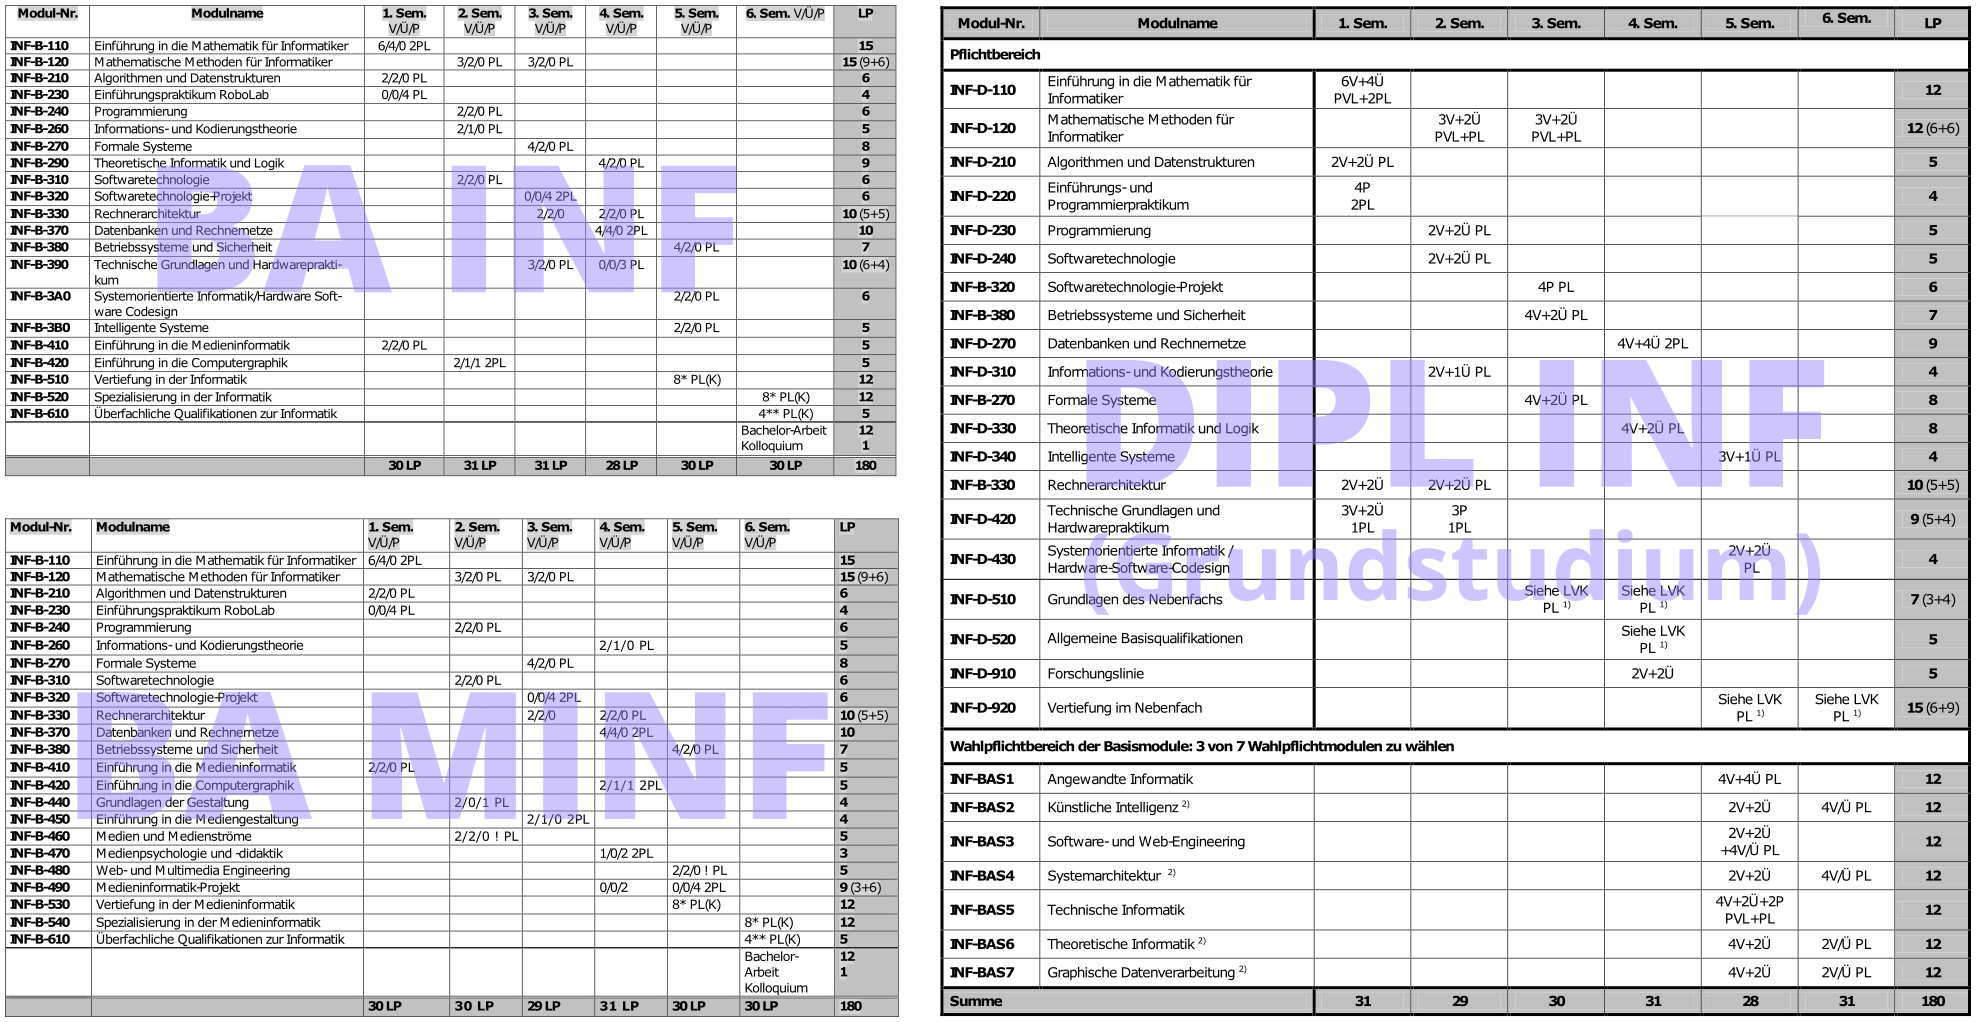
\includegraphics[width=\textwidth]{img/alle_studienablaufplaene.png}
	\caption*{\small \textit{Die Studienablaufpläne aller Studiengänge findest du in groß unter}~\link{https://tu-dresden.de/ing/informatik/studium/studienangebot}.}
\end{figure}

\minisec{Vorlesung}

In der Vorlesung wird der Stoff vermittelt, der schlussendlich in der Prüfung abgefragt wird. 
Es ist also sinnvoll, die Vorlesung aktiv zu verfolgen und sie ggf. vor- und nachzubereiten. 
Nicht ratsam ist es, erst vor der Prüfung den ganzen Stoff aufzuholen, da die Stoffmenge in der Regel sehr groß ist und es also unnötig mehr Stress in der Prüfungsphase bedeuten würde. \\
Besonders am Anfang deines Studium ist die Zahl der Zuhörer einer Vorlesung im dreistelligen Bereich. 
Daran gewöhnt man sich aber in der Regel schnell.
Je mehr Leute aber in einer Vorlesung sitzen, desto Wahrscheinlicher ist es, dass jemand an einer Stelle in der Vorlesung nicht mitkommt. 
Das kann jedem mal passieren.
Falls du also dieser jemand sein solltest, habe keine falsche Scheu, den Dozierenden eine Frage zu stellen, um die Unklarheiten zu beseitigen. 
Aktive Beteildigung in der Vorlesung ist immer gerne gesehen bei den Dozierenden.
Und ja, auch wenn es eine Verständnisfrage ist. 
Wahrscheinlich freut sich dann auch der ein oder andere Kommilitone von dir, der dieselbe Frage, aber nicht den Mut hatte zu fragen. \\
Welche Vorlesung du in welchem Semester besuchen solltest, findest du im jeweiligen Studienablaufplan deines Studiengangs
(Bachelor Informatik~\link{https://www.verw.tu-dresden.de/AmtBek/PDF-Dateien/2016-06/11soBA24.04.2016.pdf}, Bachelor Medieninformatik~\link{https://www.verw.tu-dresden.de/AmtBek/PDF-Dateien/2016-06/11soBAMI24.04.2016.pdf}, Diplom Informatik~\link{https://tu-dresden.de/die_tu_dresden/fakultaeten/fakultaet_informatik/studium/dateien/studien_und_pruefungsordnungen/dipl_inf_so_app1_de.pdf}) oder im Vorlesungsverzeichnis auf der Seite der Fakultät~\link{https://tu-dresden.de/ing/informatik/studium/lehre}. 


\minisec{Übung}

Übungen werden zu fast allen Vorlesungen angeboten und dienen dazu, Aufgaben zum aktuellen Vorlesungsstoff zu bearbeiten. Klausuren orientieren sich häufig an den Übungsaufgaben, deshalb solltest du die Übungen
regelmäßig besuchen. Die Übungen werden meistens von Studenten aus höheren Semestern oder von Lehrstuhlmitarbeitern gehalten, nicht vom Professor.
Das hat auch den Vorteil, dass man bekanntlich viele Dinge besser versteht, wenn man sie noch einmal aus einem anderen Mund erklärt bekommt.
Die jeweils aktuellen Übungsaufgaben findest du auf der Seite des jeweiligen Dozenten, oft unter den Stichworten Teaching oder Lehre.
Es wird erwartet, dass du dir die Aufgaben bereits vor der Übung anschaust, um dann Lösungen oder Fragen zu diskutieren.


\minisec{Praktikum}

Das erste Praktikum erwartet dich bereits in der vorlesungsfreien Zeit des ersten Semesters -- plane deinen Urlaub also lieber nicht zu schnell!
Dort wirst du im Einführungspraktikum \textit{Robolab} dein Können unter Beweis stellen. Diplomer müssen zusätzlich noch das Strategiespielepraktikum absolvieren.
Ein ganzes Praktikumssemester ist nur für Diplomstudenten im 7. Semester Pflicht.
Natürlich ist es trotzdem empfehlenswert, Praktika bei echten Firmen außerhalb der Fakultät in den Semesterferien zu machen, das steigert nicht nur deine Jobchancen,
sondern zeigt dir auch, ob deine Studienwahl tatsächlich die Richtige war.

\refstepcounter{dummy}\label{sec:pruefungen}
\minisec{Prüfungen}
Direkt an die Vorlesungszeit schließt die Prüfungszeit an – die wohl stressigste Zeit im Leben eines Studenten.
Die genauen Prüfungstermine findest du für das Wintersemester meist etwa Anfang Januar auf der Homepage der Fakultät~\link{https://tu-dresden.de/ing/informatik/studium/news} oder direkt beim Prüfungsamt~\link{https://tu-dresden.de/ing/informatik/studium/pruefungsorganisation}.
Im Laufe des Semesters hast du die Gelegenheit, dich dafür (innerhalb der Einschreibefrist) über jExam einzuschreiben.
Dort hast du auch die Möglichkeit, dich bis zu drei \emph{Werk}tage vor der Prüfung wieder auszutragen. Du kannst die Prüfung auch in einem späteren Semester schreiben. Das sollte aber natürlich nicht zum Regelfall werden. Für mündliche und sonstige Prüfungen gilt eine Abmeldefrist von 14 Tagen.
Solltest du aufgrund eines Rücktritts innerhalb der Frist oder einer plötzlichen Erkrankung von der Prüfung ausscheiden, kannst du dich auf der Seite des Prüfungsamtes informieren,
welche Nachweise (Atteste) du im Prüfungsamt innerhalb welcher Frist einreichen musst~\link{https://tu-dresden.de/ing/informatik/studium/pruefungsorganisation/pruefungen/abmelden-ruecktritt-krankheit}.
Prüfungen werden mit Noten bewertet, wobei alle mit besser als 5.0 bewerteten Prüfungen als bestanden gelten und nicht wiederholt werden können.
Noten Schlechter als 5.0 gibt es nicht.
Die 5.0 ist damit die einzige Chance, eine Prüfung nicht zu bestehen.
Hast du das erst einmal geschafft, gibt es die Möglichkeit, die Prüfung innerhalb von zwei Semestern zu wiederholen.
Nach dem zweiten nicht geglückten Prüfungsversuch hast du nur noch ein Semester Zeit bis der dritte erfolgen muss.
Erst wenn du das dritte Mal die Klausur nicht bestanden hast (also die zweite Wiederholungsklausur), wirst du exmatrikuliert.
Genauere Informationen zu dieser Thematik findest du stets in der Prüfungs- bzw.\ der Studienordnung, die du dir unbedingt mal angeschaut haben solltest.
Deine erste Matheprüfung erwartet dich übrigens bereits im Dezember: die sogenannte Nikolausklausur.

\begin{figure}
	\begin{tikzpicture}
		\draw (0,0) rectangle (4,-5);
		\draw (0,0) [fill=black] rectangle (4, -.5);
		\node at (2,0) [below] {\textcolor{white}{Die meisten Module:}};
		\draw (0,-.5) [fill=gray!40] rectangle (4,-1);
		\node at (2,-.5) [below] {bspw. AuD};
		\draw (0,-.5) -- (4,-.5);
		\node (v1) [draw] at (2,-1.6) {Vorlesung};
		\node (u1) [draw] at (2,-2.7) {Übung};
		\draw (0,-3.5) -- (4,-3.5);
		\node (p1) [draw] at (2,-4.3) {Prüfung};

		\draw (5,0) rectangle (12, -5);
		\draw (5,0) [fill=black] rectangle (12, -.5);
		\node at (8.5,0) [below] {\textcolor{white}{Spezialfall Mathe im 1. Semester:}};
		\draw (5,-.5) -- (12,-.5);
		\node (pvl) [rectangle,draw,font=\scriptsize] at (8.5,-3.3) [above]{Hausaufgaben};
		\draw (8.5,-.5) -- (pvl);
		\draw (5,-.5) [fill=gray!40] rectangle (8.5,-1);
		\node at (6.75,-.5) [below] {LAG};
		\draw (8.5,-.5) [fill=gray!40] rectangle (12,-1);
		\node at (10.25,-.5) [below] {DIS};
		\draw (5,-1) -- (12, -1);
		\node (v2) [draw] at (6.6,-1.6) {Vorlesung};
		\node (u2) [draw] at (6.1,-2.7) {Übung};
		\node (v3) [draw] at (10.1,-1.6) {Vorlesung};
		\node (u3) [draw] at (10.9,-2.7) {Übung};
		\draw (5,-3.3) -- (12,-3.3);
    \node (p2) [draw] at (7.35,-4) {\enquote{Nikolausprüfung}};
		\node (p3) [draw] at (10.7,-4.4) {Prüfung};
		%\draw[->,thick] (pvl) -- (p3);
	\end{tikzpicture}
\end{figure}

\newpage

\minisec{Leistungsnachweis}

Bei manchen Prüfungen erhältst du neben der Note einen Leistungsnachweis (oder kurz: Schein).
Dazu zählen unter anderem die Sprachkurse, die Forschungslinie und z.T. Nebenfachprüfungen. Diese Scheine brauchst du, um dir diese Leistungen im Prüfungsamt anrechnen lassen zu können.

\refstepcounter{dummy}\label{sec:sprachausbildung}
\minisec{Sprachausbildung}

Es werden an der TU Dresden Kurse für fast alle möglichen (und unmöglichen) Sprachen angeboten.
Zu diesem Zweck gibt es zwei Zentren für die Sprachausbildung: Das \enquote{Lehrzentrum Sprachen und Kulturen} (LSK) und \enquote{TUD Institute of Advanced Studies} (TUDIAS).
Das Sprachangebot der beiden Einrichtungen ähnelt sich sehr stark.
Du hast für diverse Sprachkurse ein Budget an Semesterwochenstunden (insgesamt 10 SWS), die du ausgeben kannst, wie du willst.
Für dein Studium zum Bachelor der (Medien-)Informatik sind Sprachkurse generell optional, aber auf jeden Fall empfehlenswert.
Für Diplomstudenten sind 2 Semester Englisch im Laufe des Studiums Pflicht.
Studierst du allerdings Bachelor Informatik und möchtest danach mit dem Master Informatik an der TU Dresden weitermachen, wirst du für den Master das Sprachniveau B2 in Englisch nachweisen müssen,
also kann es sich auch für dich anbieten, die entsprechenden Sprachkurse zu besuchen.
Die Einschreibung für einen Sprachkurs erfolgt online~\link{https://sprachausbildung.tu-dresden.de} mit deinem ZIH-Login.
Sobald die Kurse freigeschaltet sind, solltest du dich jedoch stark beeilen, denn die beliebten Kurse sind meist innerhalb weniger Minuten voll.
Weitere Infos findest du unter~\link{https://tu-dresden.de/lsk}~und~\link{https://www.tudias.de/}.

\vfill
\begin{center}
  \includegraphics[trim={0 4cm 0 0}, clip, width=\linewidth]{img/ese2013/foyer.jpg}
\end{center}

\minisec{Schreibberatung}
Das Schreibzentrum der TU Dresden~\link{https://www.facebook.com/SchreibzentrumTUD} ist ein Kooperationsprojekt für Studierende und Lehrende vom Zentrum für Weiterbildung und dem Career Service. Es bietet Unterstützung, Methoden und Ideen zum Thema \enquote{wissenschaftliches Schreiben}.
Du kannst mit deinen Schreibprojekten aller Art (Beleg, Seminararbeit, Abschlussarbeit, etc.) entweder in die offene Schreibsprechstunde am SCS ServicePoint der SLUB kommen oder einen individuellen Termin per E-Mail~\link{mailto:Schreibzentrum@mailbox.tu-dresden.de} vereinbaren.
Dabei spielt es keine Rolle, wie weit die Arbeit bereits ist, ob man also noch ganz am Anfang steht oder kurz vor der Abgabe.
Auch muss kein konkretes Problem vorliegen, sondern intuitive Anliegen zur Arbeit können ebenfalls geschildert werden.

Die Schreibberatung unterstützt bei Fragen zum Schreibprozess -- von der Themenfindung, über die Gliederung bis hin zur Abgabe der fertigen Arbeit.
Ausgebildete studentische Schreibtutorinnen und Schreibtutoren unterstützen dich mit vielfältigen Schreibmethoden und Techniken.
Inhaltliche Tipps oder Hilfestellungen können dir dabei nicht gegeben werden.
Auch liest die Schreibberatung keine Texte Korrektur; allerdings kannst du exemplarisch Textfeedback auf Textauszüge bekommen.
Das Angebot ist selbstverständlich kostenlos.

\minisec{Stipendien}

Neben dem BAföG sind auch Stipendien eine gern genutzte Möglichkeit der Studienfinanzierung.

Viele Stipendien werden von den 13 überwiegend staatlich finanzierten Begabtenförderungswerken vergeben, die sich hinsichtlich ihres weltanschaulichen, religiösen oder politischen Profils unterscheiden.
Oftmals werden Studierende aufgrund guter Leistungen von Schulen, Prüfungsämtern oder Hochschullehrern direkt vorgeschlagen.
Bei vielen Werken sind aber auch Selbstbewerbungen möglich.
Für die Aufnahme muss man keineswegs ein Überflieger sein.

Im Auswahlprozess können gesellschaftliches oder soziales Engagement eine ebenso wichtige Rolle spielen.
Die Stipendien werden in Anlehnung an das BAföG abhängig vom eigenen Einkommen und Vermögen sowie vom Einkommen der Eltern berechnet.
Zusätzlich erhalten die Stipendiaten eine monatliche Studienkostenpauschale in Höhe von 300 Euro.
Im Gegensatz zum BAföG müssen die Stipendien jedoch nicht zurückgezahlt werden.
Neben der finanziellen Förderung bieten alle Werke eine umfangreiche ideelle Förderung in Form von Sprachkursen, Exkursionen und Akademien.

Ebenso bekannt ist das Deutschlandstipendium, welches zur Hälfte von privaten Geldgebern finanziert wird.
Die finanzielle Förderung erfolgt unabhängig vom eigenen Einkommen oder dem der Eltern und beläuft sich auf 300 Euro monatlich.
Das Deutschlandstipendium wird nicht auf das BAföG angerechnet und muss ebenfalls nicht zurückgezahlt werden.
Bewerbungen werden jeweils im Juli direkt vom Zentrum für Weiterbildung der TU Dresden~\link{https://tu-dresden.de/deutschlandstipendium} entgegengenommen.

Es gibt noch viele weitere Organisationen, deren Förderung überwiegend privat finanziert wird. Diese vergeben jedoch oft nur wenige Vollstipendien oder beschränken die Förderung auf geringere Sach- oder Geldleistungen.

\begin{figure}[b]
	\centering
	\includegraphics[width=\textwidth, keepaspectratio]{img/xkcd/zealous_autoconfig.png}
	\caption*{{\small \textit{I hear this is an option in the latest Ubuntu release. (https://xkcd.com/416)}}}
\end{figure}

\minisec{Hochschulgruppen}
\label{sec:hsg}

Lernen und feiern reicht dir nicht?
Such dir eine Hochschulgruppe!
Dort findest du ehrenamtlich engagierte Studierende, die aktiv das Leben auf
dem Campus mitgestalten wollen.
Und je nachdem was du suchst, wirst du auch Diskussionen, die Möglichkeit anderen zu helfen, neue Erfahrungen, interessante Leute und vieles mehr finden können.

Thematisch ist für jeden etwas dabei.
So gibt es Hochschulgruppen mit politischem und gesellschaftlichem Engagement.
Andere sind interessiert an der Gestaltung kultureller Vielfalt in Dresden.
Natürlich sind aber auch technisch orientierte Hochschulgruppen vertreten.
Schau dich einfach mal hier~\link{https://www.stura.tu-dresden.de/hochschulgruppen} um und melde dich direkt bei einer Hochschulgruppe deiner Wahl.
Vielleicht ist ja was für dich dabei.

\minisec{Auslandsaufenthalte}

Bei akutem Auslandswunsch oder studienbegleitendem Internationalisierungsdrang fragen Sie bitte das Auslandsamt der Uni oder Ihren Professor des Vertrauens.
Auslandsaufenthalte können Nebenwirkungen hervorrufen.
Über diese können Sie sich bei Kommilitonen erkundigen.

Im Verlaufe deines Studiums werden dich immer wieder Leute fragen, ob du nicht ein oder zwei Semester im Ausland verbringen möchtest.
Nun magst du dich als unschuldiger Erstsemester fragen, warum denn das und wieso kommt ihr jetzt schon damit an?
Die Antwort ist einfach:
Zum einen kannst du direkt deine Sprachkenntnisse verbessern, Kontakte knüpfen und neue Kulturen erleben -- Eine willkommene Abwechslung, um den Kopf frei zu bekommen nach den anstrengenden Semestern. Es werden neue Perspektiven vermittelt, sowohl akademisch als auch fachlich. Außerdem hilft es dir bei der Entwicklung deiner Softskills wie Selbstständigkeit, Toleranz und Anpassungsfähigkeit (um nur einige zu nennen). Alles Dinge, die dir später weiterhelfen werden und für die du später dankbar sein wirst.
Kurz und knapp gesagt ein Auslandsaufenthalt ist nützlich, erfordert aber etwas Planung.
Deshalb ist es von Vorteil sich möglichst früh zu informieren.
Für Infos und bei Fragen kannst du dich an das Akademische Auslandsamt (AAA) der TU~\link{https://tu-dresden.de/studium/im-studium/beratung-und-service/akademisches-auslandsamt} wenden und auf den Seiten der Fakultät~\link{https://tu-dresden.de/ing/informatik/studium/internationales/outgoing} informieren.
Wenn man mutig ist, kann man sogar Professoren direkt fragen, ob sie Kontakte zu anderen Unis oder Unternehmen haben.
Es liegt an dir, wie erfolgreich dein Auslandsaufenthalt wird.
Ob beim Streicheln von Robben vor Neufundland oder beim Scrum-Meeting im Silicon Valley, es gibt eine Menge Angebote, die auf dich warten!

% \begin{figure}[b!]
% 	\centering
% 	\includegraphics[width=0.9\linewidth]{img/ese2014/einschreibung.jpg}
% \end{figure}%

\minisec{Urlaubssemester}
Es gibt eine ganze Reihe von Gründen, die dich daran hindern können, dein Studium an der TU ordnungsgemäß weiterzuführen.
Klassische Gründe sind schwere Erkrankungen, längere Praktika, Auslandsaufenthalte oder (unverhoffter) Nachwuchs, um den du dich kümmern musst.
In solchen Fällen kannst du dich von deinem Studium beurlauben lassen, um dich voll und ganz auf den Urlaubsgrund zu konzentrieren.
Während eines Urlaubssemesters bist du von der Pflicht befreit, Prüfungen ablegen zu müssen, genießt aber weiterhin alle Vorteile des Studierendendaseins.
Andererseits hast du in dieser Zeit meist auch keinen Anspruch auf BAföG- oder Kindergeld-Zahlungen, also plane das nicht unbedingt bei deinen Einkünften ein.

Solltest du ein Auslandsstudium machen und ein paar Semester in fernen Landen verweilen, kannst du dir danach erbrachte Leistungen und Prüfungen hier anrechnen lassen.
Einziger Fallstrick dabei: Wenn du genügend Leistungspunkte einbringst, wirst du trotzdem ein Fachsemester hochgestuft, aber da kann dir die Studienfachberatung weiterhelfen.

Beantragen kannst du ein Urlaubssemester beim Immatrikulationsamt~\link{https://tu-dresden.de/imma/} während der Rückmeldefrist für das nächste Semester.
Wie genau das geht und weitere Informationen findest du unter~\link{https://tu-dresden.de/studium/im-studium/studienorganisation/beurlaubung}.

\include{texte/moduluebersicht}
\include{texte/werbung}
\addchap{Links}

Alle Links sind auch direkt als \url{https://ese.ifsr.de/\eseyear/<Zahl>} aufrufbar.

{%
\small
\begin{longtable}{r p{11cm}}
\linklist%
\end{longtable}
}


% \addchap{Notizen}\mbox{}
%\cleardoubleevenemptypage

\ifcase\numexpr \modulo{\value{page}}{2} \relax
% don't add any extra pages
\or
\hbox{}
\vspace{5mm}
\begin{center}
\tiny
--- This page is unintentionally left blank ---
\vfill
:P
\end{center}
\newpage
\fi


\addchap{Rätsel}

Kennst du Picross oder Nonogramm (oder eine ganze Sammlung von weiteren Begriffen)?
In diesem Logikrätsel ist ein Pixelbild versteckt.
An jeder Zeile und Spalte steht nur, wie viele aufeinanderfolgende ausgefüllte Pixel es in der Reihe gibt.
Dazwischen können jeweils beliebig viele unausgefüllte liegen.

\vfill
% no centering, the image is already off center because the numbers are only on one side of the grid
\includegraphics[width=.95\textwidth]{raetsel/picross}

\vspace{3mm}


\pagebreak

Es sind die 1960er Jahre, du arbeitest mit einem Kommilitonen an einem ersten Prototypen für miteinander vernetzte Computer.
Der Algorithmus ist noch recht simpel.
Zu simpel: denn jeder Rechner schickt von einer Verbindung in der einen Sekunde empfangene Nachrichten in der nächsten Sekunde einfach blind an alle anderen Verbindungen weiter.
Wenn eine Nachricht aber gleichzeitig aus mehr als einer Verbindung eingeht,
 crasht der Rechner und ist erst in der nächsten Sekunde wieder einsatzfähig --
 ohne das soeben Empfangene weiterzusenden.
\\
Du versuchst natürlich, deinem Kommilitonen das als Nachricht auf den einzigen Rechner mit aktivierten Logs zu schicken.
Aber den zu erreichen gestaltet sich erstaunlich schwierig,
 denn du hast nur ein Kabel, und es reicht nur zu drei anderen Rechnern...
Mit welcher Verbindung kommt die Nachricht sicher ans Ziel -- ohne dieses zu crashen?

\vfill%

\begin{minipage}{.2\textwidth}
\vfill

\[t\]

\begin{tikzpicture}[
    every node/.style={circle, draw, fill=black, inner sep=1pt, minimum size=2.5mm},
]
  \node [double] (a) at  (0.5, 0.25)  {}  edge    [<-]        (0,0.25);
  \node []       (b) at  (1.25,0   )  {}  edge    [-]         (a)
                                          edge    [-]         (1.75,0);
  \node []       (c) at  (1.25,0.5 )  {}  edge    [-]         (a)
                                          edge    [-]         (1.75,0.5);
\end{tikzpicture}

\vspace{1mm}

\[t+1\]

\begin{tikzpicture}[
    every node/.style={circle, draw, fill=black, inner sep=1pt, minimum size=2.5mm},
]
  \node []       (a) at  (0.5, 0.25)  {}  edge    [-]         (0,0.25);
  \node [double] (b) at  (1.25,0   )  {}  edge    [<-]        (a)
                                          edge    [-]         (1.75,0);
  \node [double] (c) at  (1.25,0.5 )  {}  edge    [<-]        (a)
                                          edge    [-]         (1.75,0.5);
\end{tikzpicture}


\vspace{6mm}


\[t\]

\begin{tikzpicture}[
    every node/.style={circle, draw, fill=black, inner sep=1pt, minimum size=2.5mm},
]
  \node [double]   (b) at  (0.5, 0   )  {}  edge    [<-]        (0,0);
  \node [double]   (c) at  (0.5, 0.5 )  {}  edge    [<-]        (0,0.5);
  \node []         (d) at  (1.25,0.25)  {}  edge    [-]         (b)
                                            edge    [-]         (c);
  \node []         (e) at  (1.75,0.25)  {}  edge    [-]         (d)
                                            edge    [-]         (2.25,0.25);
\end{tikzpicture}

\vspace{1mm}

\[t+1\]

\begin{tikzpicture}[
    every node/.style={circle, draw, fill=black, inner sep=1pt, minimum size=2.5mm},
    cross/.style={path picture={
      \draw[black]
    (path picture bounding box.south east) -- (path picture bounding box.north west) (path picture bounding box.south west) -- (path picture bounding box.north east);
	}},
    crashed/.style={draw, cross, thick, fill=none},
]
  \node []         (b) at  (0.5, 0   )  {}  edge    [-]         (0,0);
  \node []         (c) at  (0.5, 0.5 )  {}  edge    [-]         (0,0.5);
  \node [crashed]  (d) at  (1.25,0.25)  {}  edge    [<-]        (b)
                                            edge    [<-]        (c);
  \node []         (e) at  (1.75,0.25)  {}  edge    [-]         (d)
                                            edge    [-]         (2.25,0.25);
\end{tikzpicture}

\vspace{1mm}

\[t+2\]

\begin{tikzpicture}[
    every node/.style={circle, draw, fill=black, inner sep=1pt, minimum size=2.5mm},
]
  \node []         (b) at  (0.5, 0   )  {}  edge    [-]         (0,0);
  \node []         (c) at  (0.5, 0.5 )  {}  edge    [-]         (0,0.5);
  \node []         (d) at  (1.25,0.25)  {}  edge    [-]         (b)
                                            edge    [-]         (c);
  \node []         (e) at  (1.75,0.25)  {}  edge    [-]         (d)
                                            edge    [-]         (2.25,0.25);
\end{tikzpicture}


\vfill

\end{minipage}%
%
\hfill%
\begin{minipage}{.75\textwidth}
\includegraphics[width=\textwidth]{raetsel/network}
\end{minipage}

%\cleardoubleevenemptypage

% ensure we are on a double page
\ifcase\numexpr \modulo{\value{page}}{2} \relax
% don't add any extra pages
\or
\hbox{}
\vspace{5mm}
\begin{center}
\tiny
--- This page is unintentionally left blank ---
\vfill
:P
\end{center}
\newpage
\fi

\addchap[Campusplan]{}
\thispagestyle{empty} %keine Seitenzahl
\AddToShipoutPicture*{\put(0,0){%
\parbox[b][\paperheight]{\paperwidth}{%
\vfill
\centering
\adjincludegraphics[height=\pageheight,keepaspectratio,trim={0 0 {.5\width} 0},clip]{img/campusplan_highlighted.pdf}%
\vfill
}}}
\mbox{}
\newpage
\thispagestyle{empty} %keine Seitenzahl
\AddToShipoutPicture*{\put(0,0){%
\parbox[b][\paperheight]{\paperwidth}{%
\vfill
\centering
\adjincludegraphics[height=\pageheight,keepaspectratio,trim={{.5\width} 0 0 0},clip]{img/campusplan_highlighted.pdf}%
\vfill
}}}
\mbox{}

\newpage
\thispagestyle{empty} %keine Seitenzahl
\color{white}

\begin{minipage}[t][\textheight][b]{.65\textwidth}
\footnotesize
\textbf{Herausgeber} \\
Fachschaftsrat Informatik der TU Dresden\\
Nöthnitzer Straße 46\\
01187 Dresden\\[1\baselineskip]

Alle verwendeten Comics von Randall Munroe (\textit{xkcd.com}) unter Creative Commons Lizenz:\\
\url{https://creativecommons.org/licenses/by-nc/2.5/}\\[1\baselineskip]

Redaktionsschluss dieser Ausgabe ist ein milder Spätsommerabend Mitte September 2021, zu Beginn der vorletzten Welle im Jahr 2021. %[1\baselineskip]
Schwankungen im inhaltlichen Umfang sind technisch bedingt.\\[1\baselineskip]

Mitarbeit an der nächsten Version,\\
Verbesserungsvorschläge oder Tippfehlerfunde\\
sind unter \url{https://github.com/fsr/nopanic}\\
immer willkommen!\\[1\baselineskip]

Powered by \LaTeX
\end{minipage}%
\hfill%
\begin{minipage}[t][\textheight][b]{.25\textwidth}
\fontsize{6pt}{7.2pt}\selectfont
\raggedleft
\textbf{Dank an:}\\[1\baselineskip]
Amelie Wagner\\
Anita Fritzsche\\
Anja Reusch\\
Bianca Güttner\\
Casey Kreer\\
Christoph Baitis\\
Elizaveta Soldatova\\
Emelie Radziwill\\
Emmanuel Diehl\\
Fabian Plichta\\
Felix Wittwer\\
Florian Kluge\\
Franka Schlösser\\
Franz Rodestock\\
Georg Gonsior\\
Hassan Abdullah\\
Hendrik Wolff\\
Jacques-Maurice Walther\\
Jakob Krebs\\
Jakob Steinberg\\
Jannusch Bigge\\
Johann Bläsche\\
Jonas Frei\\
Jonas Gaffke\\
Julius Hanusch\\
Katja Linnemann\\
Laila Walter\\
Linus Wemmer\\
Lokesh Kumar\\
Lydia Will\\
Marco Lehner\\
Muhammad Sarmad Aidrus\\
Moritz Uhlig\\
Ngoc Nguyen\\
Niklas Keerl\\
Noemi Ernst\\
Ole Voß\\
Oliver Scholz\\
Otto Soyka\\
Patrik Phan\\
Per Natzschka\\
Philipp Freytag\\
Pius \foreignlanguage{english}{\enquote{\TeX}} Meinert\\
Rebecca Uecker\\
Sabrina \foreignlanguage{english}{\enquote{soon PhD}} Mielke\\
Sebastian Heiden\\
Simon Birkenheuer\\
Sofia Kaltwasser\\
Till Dirschnabel\\
Tassilo Tanneberger\\
Tobias Maschek\\
Tobias Neubauer\\
Undine Stelter\\
Viktor Reusch\\
Vincent Melisch\\
Weronika Laßnack\\
Yorick Behme\\
\end{minipage}

\enlargethispage{2\baselineskip}

\newcommand\BackcoverPic{%
\put(0,0){%
\parbox[b][\paperheight]{\paperwidth}{%
\vfill
\centering
\includegraphics[width = \paperwidth, height = \paperheight]{cover/Hinten}%
\vfill
}}}
\AddToShipoutPicture*{\BackcoverPic}


% Always close your files :)
\immediate\closeout\linklistfile

\end{document}
